\chapter{Continuous Functions} \label{lim:chapter}

%%%%%%%%%%%%%%%%%%%%%%%%%%%%%%%%%%%%%%%%%%%%%%%%%%%%%%%%%%%%%%%%%%%%%%%%%%%%%%

\section{Limits of functions}
\label{sec:limoffunc}

\sectionnotes{2--3 lectures}

Before we define continuity of functions, we need to visit a somewhat
more general notion of a limit.  That is, given a function $f \colon S \to
\R$, we want to see how $f(x)$ behaves as $x$ tends to a certain point.

\subsection{Cluster points}

First,
let us return to a concept we have previously seen in an exercise.

\begin{defn}
Let $S \subset \R$ be a set.  A number $x \in \R$ is called
a \emph{\myindex{cluster point}} of $S$
if for every $\epsilon > 0$, the set $(x-\epsilon,x+\epsilon) \cap S
\setminus \{ x \}$ is not empty.
\end{defn}

That is, $x$ is a cluster point of $S$ if there are points of $S$
arbitrarily close to $x$.  Another way of phrasing the definition is to say
that $x$ is a cluster point of $S$ if for every $\epsilon > 0$, there
exists a $y \in S$ such that $y \not= x$ and $\abs{x - y} < \epsilon$.
Note that a cluster point of $S$ need not lie in $S$.

Let us see some examples.
\begin{enumerate}[(i)]
\item The set
$\{ \nicefrac{1}{n} : n \in \N \}$ has a unique cluster point zero.
\item The cluster points of the open interval $(0,1)$ are
all points in the closed interval $[0,1]$.
\item For the set $\Q$, the set of
cluster points is the whole real line $\R$.
\item For the set $[0,1) \cup \{ 2 \}$,
the set of cluster points is the interval $[0,1]$.
\item The set $\N$ has no cluster points in $\R$.
\end{enumerate}

\begin{prop}
Let $S \subset \R$.  Then $x \in \R$ is a cluster point of $S$
if and only if
there exists a convergent sequence of numbers $\{ x_n \}$ such that
$x_n \not= x$ and $x_n \in S$ for all $n$, and $\lim\, x_n = x$.
\end{prop}

\begin{proof}
First suppose $x$ is a cluster point of $S$.
For any $n \in \N$, we pick $x_n$ to be an arbitrary point of
$(x-\nicefrac{1}{n},x+\nicefrac{1}{n}) \cap S \setminus \{x\}$, which
we know is nonempty because $x$ is a cluster point of $S$.
Then
$x_n$ is within $\nicefrac{1}{n}$ of $x$, that is,
\begin{equation*}
\abs{x-x_n} < \nicefrac{1}{n} .
\end{equation*}
As $\{ \nicefrac{1}{n} \}$ converges to zero, $\{ x_n \}$ converges to $x$.

On the other hand, if we start with a sequence of numbers $\{ x_n \}$ in $S$
converging to $x$ such that $x_n \not= x$ for all $n$, then for every
$\epsilon > 0$ there is an $M$ such that in particular $\abs{x_M - x} <
\epsilon$.  That is, $x_M \in (x-\epsilon,x+\epsilon) \cap S \setminus \{x\}$.
\end{proof}

\subsection{Limits of functions}

If a function $f$ is defined on a set $S$ and $c$ is a cluster point of $S$,
then we define the limit of $f(x)$ as $x$ gets close to $c$.  
It is irrelevant for the definition if $f$ is defined at $c$ or not.
Furthermore, even if the function is defined at $c$, the limit of the
function as $x$ goes to $c$ can very well be different
from $f(c)$.

\begin{defn}
\index{limit of a function}%
Let $f \colon S \to \R$ be a function and $c$ a cluster point of $S$.
Suppose there exists an $L \in \R$ and for every $\epsilon > 0$,
there exists a $\delta > 0$ such that whenever $x \in S \setminus \{ c \}$
and $\abs{x - c} < \delta$, then
\begin{equation*}
\abs{f(x) - L} < \epsilon .
\end{equation*}
In this case we say $f(x)$ \emph{\myindex{converges}} to $L$ as $x$ goes
to $c$.  We say $L$ is the \emph{\myindex{limit}} of $f(x)$ as $x$
goes to $c$.  We write
\begin{equation*}
\lim_{x \to c} f(x) := L ,
\end{equation*}
or 
\begin{equation*}
f(x) \to L \quad\text{as}\quad x \to c .
\end{equation*}
If no such $L$ exists, then we say that the limit does not exist or
that $f$ \emph{\myindex{diverges}} at $c$.
\end{defn}

Again the notation and language we are using above assumes the limit
is unique even though we have not yet proved that.
Let us do that now.

\begin{prop}
Let $c$ be a cluster point of $S \subset \R$ and let $f \colon S \to \R$
be a function such that $f(x)$ converges as $x$ goes to $c$.  Then
the limit of $f(x)$ as $x$ goes to $c$ is unique.
\end{prop}

\begin{proof}
Let $L_1$ and $L_2$ be two numbers that both satisfy the definition.
Take an $\epsilon > 0$ and find a $\delta_1 > 0$ such that
$\abs{f(x)-L_1} < \nicefrac{\epsilon}{2}$ 
for all $x \in S \setminus \{c\}$ with $\abs{x-c} < \delta_1$.
Also find $\delta_2 > 0$ such that
$\abs{f(x)-L_2} < \nicefrac{\epsilon}{2}$
for all $x \in S \setminus \{c\}$ with $\abs{x-c} < \delta_2$.
Put $\delta := \min \{ \delta_1, \delta_2 \}$.  Suppose $x \in S$,
$\abs{x-c} < \delta$, and $x \not= c$.  As $\delta > 0$ and $c$ is a cluster
point, such an $x$ exists.  Then
\begin{equation*}
\abs{L_1 - L_2} =
\abs{L_1 - f(x) + f(x) - L_2} \leq
\abs{L_1 - f(x)} + \abs{f(x) - L_2} < \frac{\epsilon}{2} + \frac{\epsilon}{2}
= \epsilon.
\end{equation*}
As $\abs{L_1-L_2} < \epsilon$ for arbitrary $\epsilon > 0$, then
$L_1 = L_2$.
\end{proof}

\begin{example}
Let $f \colon \R \to \R$ be defined as $f(x) := x^2$.  Then
\begin{equation*}
\lim_{x\to c} f(x) = \lim_{x\to c} x^2 = c^2 .
\end{equation*}

Proof: First let $c$ be fixed.  Let $\epsilon > 0$ be given.  Take
\begin{equation*}
\delta := \min \left\{ 1 , \, \frac{\epsilon}{2\abs{c}+1} \right\} .
\end{equation*}
Take $x \not= c$ such that $\abs{x-c} < \delta$.  In particular,
$\abs{x-c} < 1$.  By reverse triangle inequality we get
\begin{equation*}
\abs{x}-\abs{c} \leq \abs{x-c} < 1 .
\end{equation*}
Adding $2\abs{c}$ to both sides we obtain
$\abs{x} + \abs{c} < 2\abs{c} + 1$.  We compute
\begin{equation*}
\begin{split}
\abs{f(x) - c^2} &= \abs{x^2-c^2} \\
&= \abs{(x+c)(x-c)} \\
&= \abs{x+c}\abs{x-c} \\
&\leq (\abs{x}+\abs{c})\abs{x-c} \\
&< (2\abs{c}+1)\abs{x-c} \\
&< (2\abs{c}+1)\frac{\epsilon}{2\abs{c}+1} = \epsilon .
\end{split}
\end{equation*}
\end{example}

\begin{example}
Define $f \colon [0,1) \to \R$ by
\begin{equation*}
f(x) := 
\begin{cases}
x & \text{if $x > 0$} , \\
1 & \text{if $x = 0$} .
\end{cases}
\end{equation*}
Then
\begin{equation*}
\lim_{x\to 0} f(x) = 0 ,
\end{equation*}
even though $f(0) = 1$.

Proof:  Let $\epsilon > 0$ be given.  Let $\delta := \epsilon$.
Then for $x \in [0,1)$, $x \not= 0$, and $\abs{x-0} < \delta$ we get
\begin{equation*}
\abs{f(x) - 0} = \abs{x} < \delta = \epsilon .
\end{equation*}
\end{example}

\subsection{Sequential limits} \label{subseq:sequentiallimits}

Let us connect the limit as defined above with limits of sequences.

\begin{lemma}\label{seqflimit:lemma}
Let $S \subset \R$ and $c$ be a cluster point of $S$.  Let $f \colon S \to
\R$ be a function.

Then
$f(x) \to L$ as $x \to c$, if and only if for every sequence $\{ x_n \}$
of numbers such that $x_n \in S \setminus \{c\}$ for all $n$,
and such that $\lim\, x_n = c$,
we have that the sequence $\{ f(x_n) \}$ converges to $L$.
\end{lemma}

\begin{proof}
Suppose 
$f(x) \to L$ as $x \to c$, and $\{ x_n \}$ is a sequence
such that
$x_n \in S \setminus \{c\}$ and
$\lim\, x_n = c$.
We wish to show that $\{ f(x_n) \}$ converges to $L$.
Let $\epsilon > 0$ be given.  Find a $\delta > 0$ such that
if $x \in S \setminus \{c\}$ and $\abs{x-c} < \delta$, then
$\abs{f(x) - L} < \epsilon$.  As
$\{ x_n \}$  converges to $c$, find an $M$ such that for $n \geq M$
we have that $\abs{x_n - c} < \delta$.  Therefore, for $n \geq M$,
\begin{equation*}
\abs{f(x_n) - L} < \epsilon .
\end{equation*}
Thus $\{ f(x_n) \}$ converges to $L$.

For the other direction, we use proof by contrapositive.  Suppose 
it is not true that $f(x) \to L$ as $x \to c$.  The negation of the
definition is that there exists an $\epsilon > 0$ such that for every
$\delta > 0$ there exists an $x \in S \setminus \{c\}$, where
$\abs{x-c} < \delta$
and $\abs{f(x)-L} \geq \epsilon$.

Let us use $\nicefrac{1}{n}$ for $\delta$ in the above statement to
construct a sequence $\{ x_n \}$.  We have
that there exists an $\epsilon > 0$ such that for every $n$,
there exists a point $x_n \in S \setminus \{c\}$, where
$\abs{x_n-c} < \nicefrac{1}{n}$
and $\abs{f(x_n)-L} \geq \epsilon$.
The sequence $\{ x_n \}$ just constructed converges to $c$, but
the sequence $\{ f(x_n) \}$ does not converge to $L$.
And we are done.
\end{proof}

It is possible to strengthen the reverse direction of
the lemma by simply stating that
$\{ f(x_n) \}$ converges without requiring a specific limit.
See \exerciseref{exercise:seqflimitalt}.

\begin{example}
$\displaystyle \lim_{x \to 0} \, \sin( \nicefrac{1}{x} )$
does not exist, but 
$\displaystyle \lim_{x \to 0} \, x\sin( \nicefrac{1}{x} ) = 0$.
See \figureref{figsin1x}.

\begin{myfigureht}
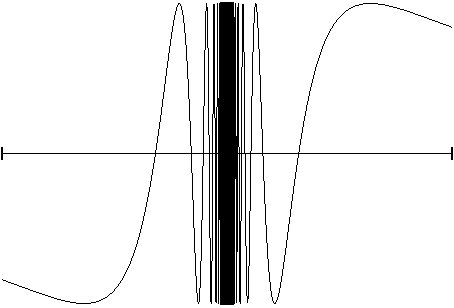
\includegraphics{figures/sin1xfig}
\qquad
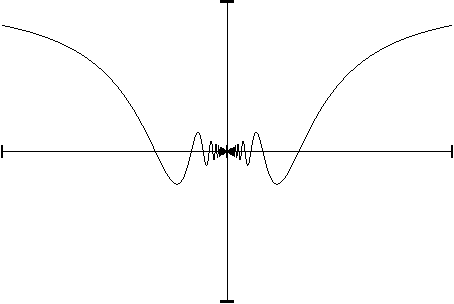
\includegraphics{figures/xsin1xfig}
\caption{Graphs of $\sin(\nicefrac{1}{x})$ and $x \sin(\nicefrac{1}{x})$.
Note that the computer cannot properly graph $\sin(\nicefrac{1}{x})$
near zero as it oscillates too fast.\label{figsin1x}}
\end{myfigureht}

Proof:
We start with $\sin(\nicefrac{1}{x})$.  Define the sequence
$x_n := \frac{1}{\pi n + \nicefrac{\pi}{2}}$.  It is not hard to see
that $\lim\, x_n = 0$.  Furthermore,
\begin{equation*}
\sin ( \nicefrac{1}{x_n} )
=
\sin (\pi n + \nicefrac{\pi}{2})
= {(-1)}^n .
\end{equation*}
Therefore, $\{ \sin ( \nicefrac{1}{x_n} ) \}$ does not converge.
Thus, by
\lemmaref{seqflimit:lemma}, 
$\lim_{x \to 0} \, \sin( \nicefrac{1}{x} )$ does not exist.

Now let us look at $x\sin(\nicefrac{1}{x})$.  Let $x_n$ be a sequence
such that $x_n \not= 0$ for all $n$, and such that $\lim\, x_n = 0$.
Notice that $\abs{\sin(t)} \leq 1$ for any $t \in \R$.  Therefore,
\begin{equation*}
\abs{x_n\sin(\nicefrac{1}{x_n})-0}
=
\abs{x_n}\abs{\sin(\nicefrac{1}{x_n})}
\leq
\abs{x_n} .
\end{equation*}
As $x_n$ goes to 0, then $\abs{x_n}$ goes to zero, and hence
$\{ x_n\sin(\nicefrac{1}{x_n}) \}$ converges to zero.  By
\lemmaref{seqflimit:lemma}, 
$\displaystyle \lim_{x \to 0} \, x\sin( \nicefrac{1}{x} ) = 0$.
\end{example}

Keep in mind the phrase ``for every sequence'' in the lemma.
For example, take $\sin(\nicefrac{1}{x})$ and the sequence $x_n = \nicefrac{1}{\pi n}$.
Then $\{ \sin (\nicefrac{1}{x_n}) \}$ is the constant zero sequence, and
therefore converges to zero.

Using \lemmaref{seqflimit:lemma}, 
we can start applying everything we know about
sequential limits to limits of functions.  Let us give a few important
examples.

\begin{cor}
Let $S \subset \R$ and $c$ be a cluster point of $S$.  Let $f \colon S \to
\R$ and $g \colon S \to \R$ be functions.
Suppose the limits of $f(x)$ and $g(x)$ as $x$ goes to $c$ both exist,
and that
\begin{equation*}
f(x) \leq g(x) \qquad \text{for all $x \in S$}.
\end{equation*}
Then
\begin{equation*}
\lim_{x\to c} f(x) \leq \lim_{x\to c} g(x) .
\end{equation*}
\end{cor}

\begin{proof}
Take $\{ x_n \}$ be a sequence of numbers in $S \setminus \{ c \}$
that converges to $c$.  Let
\begin{equation*}
L_1 := \lim_{x\to c} f(x), \qquad \text{and} \qquad L_2 := \lim_{x\to c} g(x) .
\end{equation*}
By \lemmaref{seqflimit:lemma} we know $\{ f(x_n) \}$ converges to
$L_1$ and $\{ g(x_n) \}$ converges to $L_2$.  We also
have $f(x_n) \leq g(x_n)$.
We obtain $L_1 \leq L_2$ using
\lemmaref{limandineq:lemma}.
\end{proof}

By applying constant functions, we get the following corollary.  The
proof is left as an exercise.

\begin{cor} \label{fconstineq:cor}
Let $S \subset \R$ and $c$ be a cluster point of $S$.  Let $f \colon S \to
\R$ be a function.  And suppose the limit of $f(x)$ as $x$ goes to $c$
exists.
Suppose there are two real numbers $a$ and $b$ such that
\begin{equation*}
a \leq f(x) \leq b \qquad \text{for all $x \in S$}.
\end{equation*}
Then
\begin{equation*}
a \leq \lim_{x\to c} f(x) \leq b .
\end{equation*}
\end{cor}

Using \lemmaref{seqflimit:lemma} in the same way as above we also get
the following corollaries, whose proofs are again left as an exercise.

\begin{cor} \label{fsqueeze:cor}
Let $S \subset \R$ and $c$ be a cluster point of $S$.  Let $f \colon S \to
\R$,
$g \colon S \to \R$, and $h \colon S \to \R$ be functions.  Suppose 
\begin{equation*}
f(x) \leq g(x) \leq h(x) \qquad \text{for all $x \in S$},
\end{equation*}
and the limits of $f(x)$ and $h(x)$ as $x$ goes to $c$ both exist, and
\begin{equation*}
\lim_{x\to c} f(x) = \lim_{x\to c} h(x) .
\end{equation*}
Then the limit of $g(x)$ as $x$ goes to $c$ exists and
\begin{equation*}
\lim_{x\to c} g(x) =
\lim_{x\to c} f(x) = \lim_{x\to c} h(x) .
\end{equation*}
\end{cor}

\begin{cor} \label{falg:cor}
Let $S \subset \R$ and $c$ be a cluster point of $S$.  Let $f \colon S \to
\R$ and
$g \colon S \to \R$ be functions. 
Suppose limits of $f(x)$ and $g(x)$ as $x$ goes to $c$ both exist.
Then
\begin{enumerate}[(i)]
\item
$\displaystyle
\lim_{x\to c} \bigl(f(x)+g(x)\bigr) = \left(\lim_{x\to c} f(x)\right) + 
\left(\lim_{x\to c} g(x)\right) .
$
\item
$\displaystyle
\lim_{x\to c} \bigl(f(x)-g(x)\bigr) = \left(\lim_{x\to c} f(x)\right) -
\left(\lim_{x\to c} g(x)\right) .
$
\item
$\displaystyle
\lim_{x\to c} \bigl(f(x)g(x)\bigr) = \left(\lim_{x\to c} f(x)\right)
\left(\lim_{x\to c} g(x)\right) .
$
\item \label{falg:cor:iv} If
$\displaystyle \lim_{x\to c} g(x) \not= 0$,
and $g(x) \not= 0$ for all $x \in S \setminus \{ c \}$, then
\begin{equation*}
\lim_{x\to c} \frac{f(x)}{g(x)} =
\frac{\lim_{x\to c} f(x)}{\lim_{x\to c} g(x)} .
\end{equation*}
\end{enumerate}
\end{cor}

\begin{cor} \label{fabs:cor}
Let $S \subset \R$ and $c$ be a cluster point of $S$.  Let $f \colon S \to
\R$ be a function and suppose the limit of $f(x)$ as $x$ goes to $c$ exists.
Then
\begin{equation*}
\lim_{x\to c} \abs{f(x)} =
\abs{\lim_{x\to c} f(x)}.
\end{equation*}
\end{cor}

\subsection{Limits of restrictions and one-sided limits}

Sometimes we work with the function defined on a subset.

\begin{defn}
Let $f \colon S \to \R$ be a function.  Let $A \subset S$.  Define the
function $f|_A \colon A \to \R$ by
\begin{equation*}
f|_A (x) := f(x)  \qquad \text{for $x \in A$}.
\end{equation*}
The function
$f|_A$ is called the \emph{\myindex{restriction}} of $f$ to $A$.
\end{defn}

The function $f|_A$ is simply the function $f$ taken on a smaller domain.
The following proposition is the analogue of taking a tail of a sequence.

\begin{prop} \label{prop:limrest}
Let $S \subset \R$, $c \in \R$, and
let $f \colon S
\to \R$ be a function.
Suppose
$A \subset S$ is such that there is some $\alpha > 0$ such that
$(A \setminus \{ c \}) \cap (c-\alpha,c+\alpha) = (S \setminus \{ c \}) \cap (c-\alpha,c+\alpha)$.
\begin{enumerate}[(i)]
\item The point $c$ is a cluster point of $A$ if and only if $c$ is a cluster point
of $S$.
\item Supposing $c$ is a cluster point of $S$, then $f(x) \to L$ as $x \to c$ if and only if
$f|_A(x) \to L$ as $x \to c$.
\end{enumerate}
\end{prop}

\begin{proof}
First, let $c$ be a cluster point of $A$.
Since $A \subset S$, then if $( A \setminus \{ c\} ) \cap
(c-\epsilon,c+\epsilon)$ is nonempty for every $\epsilon > 0$,
then $( S \setminus \{ c\} ) \cap
(c-\epsilon,c+\epsilon)$ is nonempty for every $\epsilon > 0$.
Thus $c$ is a cluster point of $S$.
Second, suppose $c$ is a cluster
point of $S$.  Then for $\epsilon > 0$ such that $\epsilon < \alpha$
we get that $( A \setminus \{ c\} ) \cap (c-\epsilon,c+\epsilon) =
( S \setminus \{ c\} ) \cap (c-\epsilon,c+\epsilon)$, which is nonempty.  This is true for all
$\epsilon < \alpha$ and hence 
$( A \setminus \{ c\} ) \cap (c-\epsilon,c+\epsilon)$ must be nonempty for all
$\epsilon > 0$.  Thus $c$ is a cluster point of $A$.

Now suppose $f(x) \to L$ as $x \to c$.  That is, for every $\epsilon > 0$
there is a $\delta > 0$ such that if $x \in S \setminus \{ c \}$
and $\abs{x-c} < \delta$, then $\abs{f(x)-L} < \epsilon$.  Because $A \subset S$,
if $x$ is in $A \setminus \{ c \}$, then $x$ is in $S \setminus \{ c
\}$, and hence $f|_A(x) \to L$ as $x \to c$.

Finally suppose $f|_A(x) \to L$ as $x \to c$.
For every $\epsilon > 0$
there is a $\delta' > 0$ such that if $x \in A \setminus \{ c \}$
and $\abs{x-c} < \delta'$, then $\bigl\lvert f|_A(x)-L \bigr\rvert < \epsilon$.
Take $\delta := \min \{ \delta', \alpha \}$.
Now suppose $x \in S \setminus \{ c \}$ and
$\abs{x-c} < \delta$.  As $\abs{x-c} < \alpha$, then $x \in A \setminus \{ c \}$,
and as $\abs{x-c} < \delta'$, 
we have $\abs{f(x)-L} = \bigl\lvert f|_A(x)-L
\bigr\rvert < \epsilon$.
\end{proof}

The hypothesis of the proposition is necessary.  For an arbitrary
restriction we generally only get implication in only one direction,
see \exerciseref{exercise:restrictionlimitexercise}.  

The usual notation for the limit is
\begin{equation*}
\lim_{\substack{x \to c\\x \in A}} f(x) := \lim_{x \to c} f|_A(x) .
\end{equation*}
The most common use of restriction with respect to limits
are the \emph{\myindex{one-sided limits}}%
\footnote{%
There are a plethora of notations for one sided limits.  E.g.\ for
$\lim\limits_{x \to c^-} f(x)$ one sees
$\lim\limits_{\substack{x \to c\\x < c}} f(x)$,
$\lim\limits_{x \uparrow c} f(x)$, or
$\lim\limits_{x \nearrow c} f(x)$.}.

\begin{defn} \label{defn:onesidedlimits}
Let $f \colon S \to \R$ be function and let $c$ be a cluster point of
$S \cap (c,\infty)$.  Then if the limit
of the restriction of $f$ to $S \cap (c,\infty)$ 
 as $x \to c$ exists, define
\begin{equation*}
\lim_{x \to c^+} f(x) := \lim_{x\to c} f|_{S \cap (c,\infty)}(x) .
\end{equation*}
Similarly if $c$ is a cluster point of 
$S \cap (-\infty,c)$ and the limit of the restriction as $x \to c$
exists, define
\begin{equation*}
\lim_{x \to c^-} f(x) := \lim_{x\to c} f|_{S \cap (-\infty,c)}(x) .
\end{equation*}
\end{defn}

The proposition above does not apply to one-sided limits.
It is possible to have one-sided limits, but no limit at a point.  For
example, define $f \colon \R \to \R$ by $f(x) := 1$ for $x < 0$ and
$f(x) :=
0$ for $x \geq 0$.  We leave it to the reader to verify that
\begin{equation*}
\lim_{x \to 0^-} f(x) = 1, \qquad
\lim_{x \to 0^+} f(x) = 0, \qquad
\lim_{x \to 0} f(x) \quad \text{does not exist.}
\end{equation*}
We have the following replacement.


\begin{prop} \label{prop:onesidedlimits}
Let $S \subset \R$ be a set such that $c$ is a cluster point
of both $S \cap (-\infty,c)$ and $S \cap (c,\infty)$, and let
$f \colon S \to \R$ be a function.  Then $c$ is a cluster point of $S$ and
\begin{equation*}
\lim_{x \to c} f(x) = L
\qquad \text{if and only if} \qquad
\lim_{x \to c^-} f(x) =
\lim_{x \to c^+} f(x) =
L .
\end{equation*}
\end{prop}

That is, a limit exists if both one-sided limits exist and are equal, and
vice-versa.  The
proof is a straightforward application of the definition of limit
and is left as an exercise.  The key point is that
$\bigl( S \cap (-\infty,c) \bigr) \cup \bigl( S \cap (c,\infty) \bigr)
= S \setminus \{ c \}$.

\subsection{Exercises}

\begin{exercise}
Find the limit or prove that the limit does not exist

\medskip

\noindent
\begin{tabular}{lllll}
a)
$\displaystyle
\lim_{x\to c} \sqrt{x}
$, for $c \geq 0$
& &
b)
$\displaystyle
\lim_{x\to c} x^2+x+1
$, for any $c \in \R$
& &
c)
$\displaystyle
\lim_{x\to 0} x^2 \cos (\nicefrac{1}{x})
$
\\
d)
$\displaystyle
\lim_{x\to 0}\, \sin(\nicefrac{1}{x}) \cos (\nicefrac{1}{x})
$
& &
e)
$\displaystyle
\lim_{x\to 0}\, \sin(x) \cos (\nicefrac{1}{x})
$ & 
\end{tabular}
\end{exercise}

\begin{exercise}
Prove \corref{fconstineq:cor}.
\end{exercise}

\begin{exercise}
Prove \corref{fsqueeze:cor}.
\end{exercise}

\begin{exercise}
Prove \corref{falg:cor}.
\end{exercise}

\begin{exercise}
Let $A \subset S$.  Show that if $c$ is a cluster point of $A$, then $c$
is a cluster point of $S$.  Note the difference from
\propref{prop:limrest}.
\end{exercise}

\begin{exercise} \label{exercise:restrictionlimitexercise}
Let $A \subset S$.  Suppose $c$ is a cluster point of $A$ and
it is also a cluster point of $S$.
Let $f \colon S \to \R$ be a function.  Show that if
$f(x) \to L$ as $x \to c$, then
$f|_A(x) \to L$ as $x \to c$.
Note the difference from
\propref{prop:limrest}.
\end{exercise}

\begin{exercise}
Find an example of a function $f \colon [-1,1] \to \R$ such that
for $A:=[0,1]$, the restriction
$f|_A(x) \to 0$ as $x \to 0$, but the limit of $f(x)$ as $x \to 0$
does not exist.  Note why you cannot apply
\propref{prop:limrest}.
\end{exercise}

\begin{exercise}
Find example functions $f$ and $g$ such that the limit of neither $f(x)$
nor $g(x)$ exists as $x \to 0$, but such that the limit of $f(x)+g(x)$ exists
as $x \to 0$.
\end{exercise}

\begin{exercise} \label{exercise:contlimitcomposition}
Let $c_1$ be a cluster point of $A \subset \R$ and $c_2$ be
a cluster point of $B \subset \R$.  Suppose 
$f \colon A \to B$ and $g \colon B \to \R$ are functions
such that
$f(x) \to c_2$ as $x \to c_1$ and
$g(y) \to L$ as $y \to c_2$.  If $c_2 \in B$ also suppose that $g(c_2) = L$.  Let $h(x) := g\bigl(f(x)\bigr)$ and show
$h(x) \to L$ as $x \to c_1$.
Hint: Note that $f(x)$ could equal $c_2$ for many $x \in A$,
see also
\exerciseref{exercise:contlimitbadcomposition}.
\end{exercise}

\begin{exercise}
Let $c$ be a cluster point of $A \subset \R$, and $f \colon A \to \R$
be a function.  Suppose for every sequence $\{x_n\}$ in $A$,
such that $\lim\, x_n = c$,
the sequence $\{ f(x_n) \}_{n=1}^\infty$ is Cauchy.  Prove that
$\lim_{x\to c} f(x)$ exists.
\end{exercise}

\begin{exercise} \label{exercise:seqflimitalt}
Prove the following stronger version of one direction of
\lemmaref{seqflimit:lemma}:
Let $S \subset \R$, $c$ be a cluster point of $S$, and $f \colon S \to
\R$ be a function.
Suppose that for every sequence $\{x_n\}$ in $S \setminus \{c\}$ such that
$\lim\, x_n = c$ the sequence $\{ f(x_n) \}$ is convergent.
Then show $f(x) \to L$ as $x \to c$ for some $L \in \R$.
\end{exercise}

\begin{exercise}
Prove \propref{prop:onesidedlimits}.
\end{exercise}

\begin{exercise}
Suppose $S \subset \R$ and $c$ is a cluster point of $S$.  Suppose $f \colon
S \to \R$ is bounded.  Show that there exists a sequence $\{ x_n \}$
with $x_n \in S \setminus \{ c \}$ and $\lim\, x_n = c$ such that
$\{ f(x_n) \}$ converges.
\end{exercise}

\begin{exercise}[Challenging] \label{exercise:contlimitbadcomposition}
Show that the hypothesis that $g(c_2) = L$ in
\exerciseref{exercise:contlimitcomposition} is necessary.  That is, find $f$
and $g$ such that $f(x) \to c_2$ as $x \to c_1$ and
$g(y) \to L$ as $y \to c_2$, but $g\bigl(f(x)\bigr)$ does not go to $L$
as $x \to c_1$.
\end{exercise}

\begin{exercise}
Show that the condition of being a cluster point is necessary to have a
reasonable definition of a limit.  That is, suppose $c$ is not a cluster
point of $S \subset \R$, and $f \colon S \to \R$ is a function.  Show that
every $L$ would satisfy the definition of limit at $c$ without the condition
on $c$ being a cluster point.
\end{exercise}

\begin{exercise}
a) Prove \corref{fabs:cor}.  b) Find an example showing that the converse of
the corollary does not hold.
\end{exercise}

%%%%%%%%%%%%%%%%%%%%%%%%%%%%%%%%%%%%%%%%%%%%%%%%%%%%%%%%%%%%%%%%%%%%%%%%%%%%%%

\sectionnewpage
\section{Continuous functions}
\label{sec:cont}

\sectionnotes{2--2.5 lectures}

You undoubtedly heard of continuous functions in your schooling.  A
high-school criterion for this concept is that a function is continuous if
we can draw its graph without lifting the pen from the paper.  While that
intuitive concept may be useful in simple situations, we require
rigor.  The following definition took three great mathematicians
(Bolzano, Cauchy, and finally Weierstrass) to get correctly and its final
form dates only to the late 1800s.

\subsection{Definition and basic properties}

\begin{defn}
Let $S \subset \R$, $c \in S$, and let $f \colon S \to \R$ be a function.
We say
that $f$ is \emph{continuous at $c$}\index{continuous at $c$}
if for every $\epsilon > 0$
there is a $\delta > 0$ such that whenever $x \in S$ and $\abs{x-c} <
\delta$, then
$\abs{f(x)-f(c)} < \epsilon$.

%\medskip

When $f \colon S \to \R$ is continuous at all $c \in S$, then we simply say
$f$ is a \emph{\myindex{continuous function}}.
\end{defn}
\begin{myfigureht}
\subimport*{figures/}{contigr.pdf_t}
\caption{For $\abs{x-c} < \delta$, $f(x)$ should be within the gray region.\label{fig:contigr}}
\end{myfigureht}

If $f$ is continuous for all $c \in A$, we say
$f$ is continuous on $A \subset S$.  It is left as an easy exercise to
show that this implies that $f|_A$ is continuous, although
the converse does not hold.

Continuity may be the most important definition to understand in analysis,
and it is not an easy one.  See \figureref{fig:contigr}.
Note that $\delta$ not only
depends on $\epsilon$, but also on $c$;  we need not pick
one $\delta$ for all $c \in S$.
It is no accident 
that the definition of continuity is similar to the definition of a
limit of a function.  The main feature of continuous functions
is that these are precisely the functions that behave nicely with limits.

\enlargethispage{\baselineskip}
\begin{prop} \label{contbasic:prop}
Let $S \subset \R$, let $f \colon S \to \R$ be a function, and let $c \in S$
be a point.
Then
%\begin{enumerate}[(i),itemsep=0.5\itemsep,parsep=0.5\parsep,topsep=0.5\topsep,partopsep=0.5\partopsep]
\begin{enumerate}[(i)]
\item If $c$ is not a cluster point of $S$, then $f$ is continuous at $c$.
\item If $c$ is a cluster point of $S$, then $f$ is continuous at $c$
if and only if the limit of $f(x)$ as $x \to c$ exists and
\begin{equation*}
\lim_{x\to c} f(x) = f(c) .
\end{equation*}
\item $f$ is continuous at $c$ if and only if for every sequence $\{ x_n \}$
where $x_n \in S$ and $\lim\, x_n = c$, the sequence $\{ f(x_n) \}$ converges
to $f(c)$.
\end{enumerate}
\end{prop}

\begin{proof}
Let us start with the first item.  Suppose $c$ is not a cluster point of
$S$.  Then there exists a $\delta > 0$
such that $S \cap (c-\delta,c+\delta) = \{
c \}$.  Therefore, for any $\epsilon > 0$, simply pick this given delta.
The only $x \in S$ such that $\abs{x-c} < \delta$ is $x=c$.  Then
$\abs{f(x)-f(c)} = \abs{f(c)-f(c)} = 0 < \epsilon$.

Let us move to the second item.
Suppose $c$ is a cluster point of $S$.  Let us first suppose
that $\lim_{x\to c} f(x) = f(c)$.  Then for every $\epsilon > 0$
there is a $\delta > 0$ such that if $x \in S \setminus \{ c \}$
and $\abs{x-c} < \delta$, then $\abs{f(x)-f(c)} < \epsilon$.
Also $\abs{f(c)-f(c)} = 0 < \epsilon$, so the definition of continuity at
$c$ is satisfied.  On the other hand, suppose $f$ is continuous
at $c$.  For every $\epsilon > 0$, there exists a $\delta > 0$
such that for $x \in S$ where $\abs{x-c} < \delta$ we have
$\abs{f(x)-f(c)} < \epsilon$.  Then the statement is, of course, still true if
$x \in S \setminus \{ c \} \subset S$.  Therefore $\lim_{x\to c} f(x) =
f(c)$.

For the third item, first suppose $f$ is continuous at $c$.  Let $\{ x_n \}$
be a sequence such that $x_n \in S$ and $\lim\, x_n = c$.  Let $\epsilon > 0$
be given.  Find a $\delta > 0$ such that $\abs{f(x)-f(c)} < \epsilon$
for all $x \in S$ where $\abs{x-c} < \delta$.  Find an $M \in \N$
such that for $n \geq M$ we have $\abs{x_n-c} < \delta$.  Then for
$n \geq M$ we have that $\abs{f(x_n)-f(c)} < \epsilon$, so $\{ f(x_n) \}$
converges to $f(c)$.

Let us prove the other direction of the third item by contrapositive.
Suppose $f$ is not
continuous at $c$.  Then there exists an $\epsilon > 0$
such that for all $\delta > 0$, there exists an $x \in S$
such that $\abs{x-c} < \delta$ and $\abs{f(x)-f(c)} \geq \epsilon$.
Let us define a sequence $\{ x_n \}$ as follows.
Let $x_n \in S$ be such that $\abs{x_n-c} < \nicefrac{1}{n}$
and $\abs{f(x_n)-f(c)} \geq \epsilon$.
Now $\{ x_n \}$ is
a sequence of numbers in $S$ such that
$\lim\, x_n = c$ and such that
$\abs{f(x_n)-f(c)} \geq \epsilon$ for all $n \in \N$.  Thus $\{ f(x_n) \}$
does not converge to $f(c)$.  It may or may not converge, but it definitely
does not converge to $f(c)$.  
\end{proof}

The last item in the proposition is particularly powerful.  It allows us to
quickly apply what we know about limits of sequences to continuous functions
and even to prove that certain functions are continuous.
It can also be strengthened, see \exerciseref{exercise:contseqalt}.

\begin{example}
$f \colon (0,\infty) \to \R$ defined by
$f(x) := \nicefrac{1}{x}$ is continuous.

Proof: Fix $c \in (0,\infty)$.  
Let $\{ x_n \}$ be a sequence in $(0,\infty)$ such that
$\lim\, x_n = c$.  Then we know that
\begin{equation*}
f(c) = \frac{1}{c}
=
\frac{1}{\lim\, x_n}
=
\lim_{n \to \infty} \frac{1}{x_n}
=
\lim_{n \to \infty} f(x_n) .
\end{equation*}
Thus $f$ is continuous at $c$.  As $f$ is continuous at all $c \in
(0,\infty)$, $f$ is continuous.
\end{example}

We have previously shown $\lim_{x \to c} x^2 = c^2$ directly.  Therefore
the function $x^2$ is continuous.  We can use the continuity of
algebraic operations with respect to limits of sequences, which we proved in
the previous chapter, to prove a much more general result.

\begin{prop}
Let $f \colon \R \to \R$ be a \emph{\myindex{polynomial}}.  That is
\begin{equation*}
f(x) = a_d x^d + a_{d-1} x^{d-1} + \cdots + a_1 x + a_0 ,
\end{equation*}
for some constants $a_0, a_1, \ldots, a_d$.
Then $f$ is continuous.
\end{prop}

\begin{proof}
Fix $c \in \R$.  
Let $\{ x_n \}$ be a sequence such that
$\lim\, x_n = c$.  Then
\begin{equation*}
\begin{split}
f(c) &=
a_d c^d + a_{d-1} c^{d-1} + \cdots + a_1 c + a_0 
\\
&= 
a_d {(\lim\, x_n)}^d + a_{d-1} {(\lim\, x_n)}^{d-1} + \cdots + a_1 (\lim\, x_n) + a_0 
\\
& =
\lim_{n \to \infty}
\left(
a_d x_n^d + a_{d-1} x_n^{d-1} + \cdots + a_1 x_n + a_0 
\right)
=
\lim_{n \to \infty}
f(x_n) .
\end{split}
\end{equation*}
Thus $f$ is continuous at $c$.  As $f$ is continuous at all $c \in \R$,
$f$ is continuous.
\end{proof}

By similar reasoning, or by appealing to \corref{falg:cor},
we can prove the following.  The details of the proof are left as an
exercise.

\begin{prop} \label{contalg:prop}
Let $f \colon S \to \R$ and $g \colon S \to \R$ be functions
continuous at $c \in S$.
\begin{enumerate}[(i)]
\item The function $h \colon S \to \R$ defined by
$h(x) := f(x)+g(x)$ is continuous at $c$.
\item The function $h \colon S \to \R$ defined by
$h(x) := f(x)-g(x)$ is continuous at $c$.
\item The function $h \colon S \to \R$ defined by
$h(x) := f(x)g(x)$ is continuous at $c$.
\item If $g(x)\not=0$ for all $x \in S$, the function $h \colon S \to \R$
defined by $h(x) := \frac{f(x)}{g(x)}$ is continuous at $c$.
\end{enumerate}
\end{prop}

\begin{example} \label{sincos:example}
The functions $\sin(x)$ and $\cos(x)$ are continuous.
In the following computations we use the sum-to-product
trigonometric identities.  We also use the simple facts that
$\abs{\sin(x)} \leq \abs{x}$, $\abs{\cos(x)} \leq 1$,
and $\abs{\sin(x)} \leq 1$.
\begin{equation*}
\begin{split}
\abs{\sin(x)-\sin(c)} & =
\abs{
2 \sin \left( \frac{x-c}{2} \right) \cos \left( \frac{x+c}{2} \right)
}
\\
& =
2
\abs{ \sin \left( \frac{x-c}{2} \right) }
\abs{ \cos \left( \frac{x+c}{2} \right) }
\\
& \leq
2
\abs{ \sin \left( \frac{x-c}{2} \right) }
\\
& \leq
2
\abs{ \frac{x-c}{2} }
= \abs{x-c}
\end{split}
\end{equation*}
\begin{equation*}
\begin{split}
\abs{\cos(x)-\cos(c)} & =
\abs{
-2 \sin \left( \frac{x-c}{2} \right) \sin \left( \frac{x+c}{2} \right)
}
\\
& =
2
\abs{ \sin \left( \frac{x-c}{2} \right) }
\abs{ \sin \left( \frac{x+c}{2} \right) }
\\
& \leq
2
\abs{ \sin \left( \frac{x-c}{2} \right) }
\\
& \leq
2
\abs{ \frac{x-c}{2} }
= \abs{x-c}
\end{split}
\end{equation*}

The claim that sin and cos are continuous follows by taking an
arbitrary sequence $\{ x_n \}$ converging to $c$, or by applying the
definition of continuity directly.  Details are left to the
reader.
\end{example}

\subsection{Composition of continuous functions}

You probably already realized that one of the basic tools in
constructing complicated functions out of simple ones is composition.
Recall that for two functions $f$ and $g$,
the composition $f \circ g$ is defined by
$(f \circ g)(x) := f\bigl(g(x)\bigr)$.
A composition of
continuous functions is again
continuous.

\begin{prop} \label{prop:compositioncont}
Let $A, B \subset \R$ and $f \colon B \to \R$ and $g \colon A \to B$ be
functions.  If $g$ is continuous at $c \in A$ and
$f$ is continuous at $g(c)$, then $f \circ g \colon A \to \R$ is continuous
at $c$.
\end{prop}

\begin{proof}
Let $\{ x_n \}$ be a sequence in $A$ such that $\lim\, x_n = c$.
As $g$ is continuous at $c$, then $\{ g(x_n) \}$ converges to $g(c)$.
As $f$ is continuous at $g(c)$, then $\{ f\bigl(g(x_n)\bigr) \}$ converges
to $f\bigl(g(c)\bigr)$.
Thus $f \circ g$ is continuous at $c$.
\end{proof}

\begin{example}
Claim: ${\bigl(\sin(\nicefrac{1}{x})\bigr)}^2$ is a continuous function on $(0,\infty)$.

Proof: First note that $\nicefrac{1}{x}$ is a continuous function on
$(0,\infty)$ and $\sin(x)$ is a continuous function on $(0,\infty)$ (actually
on all of $\R$, but $(0,\infty)$ is the range for $\nicefrac{1}{x}$).
Hence the composition $\sin(\nicefrac{1}{x})$ is continuous.  We also
know that $x^2$ is continuous on the interval $(-1,1)$ (the range of sin).  Thus
the composition
${\bigl(\sin(\nicefrac{1}{x})\bigr)}^2$ is also continuous on $(0,\infty)$.
\end{example}

\subsection{Discontinuous functions}

When $f$ is not continuous at $c$, we
say $f$ is \emph{\myindex{discontinuous}} at $c$, or that it has a
\emph{\myindex{discontinuity}} at $c$.
The following proposition is a useful test and follows immediately
from third item of \propref{contbasic:prop}.

\begin{prop}
Let $f \colon S \to \R$ be a function and $c \in S$.  Suppose 
there exists a sequence $\{ x_n \}$, $x_n \in S$, and $\lim\, x_n = c$
such that $\{ f(x_n) \}$ does not converge to $f(c)$.  Then $f$ is 
discontinuous at $c$.
\end{prop}

Again, 
$\{ f(x_n) \}$ may or may not converge, but
if it does, it definitely does not converge to
$f(c)$.

\begin{example} \label{example:jumpdiscont}
The function $f \colon \R \to \R$ defined by
\begin{equation*}
f(x) := 
\begin{cases}
-1 & \text{ if $x < 0$,} \\
1 & \text{ if $x \geq 0$,}
\end{cases}
\end{equation*}
is not continuous at 0.

Proof: Take the sequence $\{ - \nicefrac{1}{n} \}$, which converges to 0.  Then
$f(-\nicefrac{1}{n}) = -1$ for every $n$,
and so
$\lim\, f(-\nicefrac{1}{n}) = -1$, but $f(0) = 1$.  See
\figureref{fig:jumpdiscont}.

\begin{myfigureht}
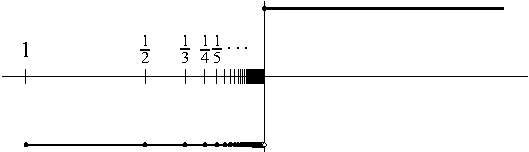
\includegraphics{figures/jumpdiscont}
\caption{Graph of the jump discontinuity.  The values of
$f(-\nicefrac{1}{n})$ and $f(0)$ are marked.\label{fig:jumpdiscont}}
\end{myfigureht}

Also notice that $f(\nicefrac{1}{n}) = 1$ for every $n$,
so $\lim \, f(\nicefrac{1}{n}) = f(0) = 1$.  So
$\{ f(x_n) \}$ may converge to $f(0)$
for some specific
sequence $\{ x_n \}$ going to 0,
despite the function being discontinuous at 0.

Finally, consider $f\bigl(\frac{{(-1)}^n}{n}\bigr) = {(-1)}^n$,
and this sequence diverges.
\end{example}

\begin{example}
For an extreme example, take the so-called
\emph{\myindex{Dirichlet function}}.
\begin{equation*}
f(x) :=
\begin{cases}
1 & \text{ if $x$ is rational,} \\
0 & \text{ if $x$ is irrational.}
\end{cases}
\end{equation*}
The function $f$ is discontinuous at all $c \in \R$.

Proof:
Suppose $c$ is rational.  Take a sequence $\{ x_n \}$
of irrational numbers such that $\lim\, x_n = c$ (why can we?).  Then $f(x_n) = 0$
and so $\lim\, f(x_n) = 0$, but $f(c) = 1$.
If $c$ is irrational, take a sequence of rational numbers $\{ x_n \}$
that converges to $c$ (why can we?).  Then $\lim\, f(x_n) = 1$, but $f(c) = 0$.
\end{example}

Let us test the limits of our intuition.  Can
there exist a function continuous at all irrational numbers, but
discontinuous at all rational numbers?  There are rational numbers
arbitrarily close to any irrational number.  Perhaps strangely, the
answer is yes.  The following example is called the
\emph{\myindex{Thomae function}}\footnote{Named after the German
mathematician
\href{http://en.wikipedia.org/wiki/Thomae}{Johannes Karl Thomae}
(1840 -- 1921).} or the
\emph{\myindex{popcorn function}}.

\begin{example} \label{popcornfunction:example}
Let $f \colon (0,1) \to \R$ be defined by
\begin{equation*}
f(x) := 
\begin{cases}
\nicefrac{1}{k} & \text{ if $x=\nicefrac{m}{k}$, where $m,k \in \N$
and $m$ and $k$ have no common divisors,} \\
0 & \text{ if $x$ is irrational}.
\end{cases}
\end{equation*}
See the graph of $f$
in \figureref{popcornfig}.
We claim that
$f$ is continuous at all irrational $c$ and 
discontinuous at all rational $c$.
\begin{myfigureht}
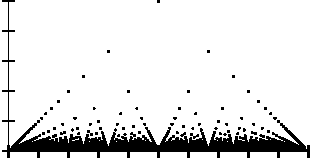
\includegraphics{figures/popcornfig}
\caption{Graph of the ``popcorn function.''\label{popcornfig}}
\end{myfigureht}

Proof:
Suppose $c = \nicefrac{m}{k}$ is rational.  Take a sequence of
irrational numbers $\{ x_n \}$ such that $\lim\, x_n = c$.  Then
$\lim\, f(x_n) = \lim \, 0 = 0$, but $f(c) = \nicefrac{1}{k} \not= 0$.  So $f$
is discontinuous at $c$.

Now let $c$ be irrational, so $f(c) = 0$.  Take a sequence 
$\{ x_n \}$ in $(0,1)$ such that $\lim\, x_n = c$.
Given $\epsilon > 0$, find $K \in \N$ such
that $\nicefrac{1}{K} < \epsilon$
by the \hyperref[thm:arch:i]{Archimedean property}.
If $\nicefrac{m}{k} \in (0,1)$ is in lowest terms
(no common divisors), then $m < k$.
So there are only finitely many rational numbers in $(0,1)$
whose denominator $k$ in lowest terms is less than $K$.  Hence
there is an $M$ such that for $n \geq M$, all the numbers $x_n$
that are rational
have a denominator larger than or equal to $K$.  Thus for $n \geq M$,
\begin{equation*}
\abs{f(x_n) - 0} = f(x_n) \leq \nicefrac{1}{K} < \epsilon .
\end{equation*}
Therefore $f$ is continuous at irrational $c$.
\end{example}

Let us end on an easier example.

\begin{example}
Define
$g \colon \R \to \R$ by $g(x) := 0$ if $x \not= 0$ and
$g(0) := 1$.  Then $g$ is not continuous at zero, but continuous everywhere else (why?).
The point $x=0$ is called a \emph{\myindex{removable discontinuity}}.  That
is because if we would change the definition of $g$, by insisting that
$g(0)$ be $0$, we would obtain a continuous function.  On the other hand
let $f$ be the function of example \exampleref{example:jumpdiscont}.
Then $f$ does not have a
removable discontinuity at $0$.  No matter how we would define $f(0)$ the function
will still fail to be continuous.  The difference is that 
$\lim_{x\to 0} g(x)$ exists while
$\lim_{x\to 0} f(x)$ does not.

Let us stay with this example but show another phenomenon.  Let $A = \{ 0
\}$, then $g|_A$ is continuous (why?), while $g$ is not continuous on $A$.
\end{example}

\subsection{Exercises}

\begin{exercise}
Using the definition of continuity directly prove that
$f \colon \R \to \R$ defined by
$f(x) := x^2$ is continuous.
\end{exercise}

\begin{exercise}
Using the definition of continuity directly prove that
$f \colon (0,\infty) \to \R$ defined by
$f(x) := \nicefrac{1}{x}$ is continuous.
\end{exercise}

\begin{exercise}
Let $f \colon \R \to \R$ be defined by
\begin{equation*}
f(x) :=
\begin{cases}
x & \text{ if $x$ is rational,} \\
x^2 & \text{ if $x$ is irrational.}
\end{cases}
\end{equation*}
Using the definition of continuity directly prove that
$f$ is continuous at $1$ and discontinuous at $2$.
\end{exercise}

\begin{exercise}
Let $f \colon \R \to \R$ be
defined by
\begin{equation*}
f(x) :=
\begin{cases}
\sin(\nicefrac{1}{x}) & \text{ if $x \not= 0$,} \\
0 & \text{ if $x=0$.}
\end{cases}
\end{equation*}
Is $f$ continuous?  Prove your assertion.
\end{exercise}

\begin{exercise}
Let $f \colon \R \to \R$ be
defined by
\begin{equation*}
f(x) :=
\begin{cases}
x \sin(\nicefrac{1}{x}) & \text{ if $x \not= 0$,} \\
0 & \text{ if $x=0$.}
\end{cases}
\end{equation*}
Is $f$ continuous?  Prove your assertion.
\end{exercise}

\begin{exercise}
Prove \propref{contalg:prop}.
\end{exercise}

\begin{exercise}
Prove the following statement.
Let $S \subset \R$ and $A \subset S$.  Let $f \colon S \to \R$
be a continuous function.
Then the restriction $f|_A$ is continuous.
\end{exercise}

\begin{exercise}
Suppose $S \subset \R$.  Suppose for some $c \in \R$
and $\alpha > 0$, we have $A=(c-\alpha,c+\alpha) \subset S$.
Let $f \colon S \to \R$ be a function.  Prove that
if $f|_A$ is continuous at $c$, then $f$ is continuous at $c$.
\end{exercise}

\begin{exercise}
Give an example of functions $f \colon \R \to \R$ and $g \colon \R \to \R$
such that the function $h$ defined by $h(x) := f(x) + g(x)$ is continuous,
but $f$ and $g$ are not continuous.  Can you find $f$ and $g$ that are nowhere
continuous, but $h$ is a continuous function?
\end{exercise}

\begin{exercise}
Let $f \colon \R \to \R$ and 
$g \colon \R \to \R$ be continuous functions.  Suppose that for
all rational numbers $r$, $f(r) = g(r)$.  Show that $f(x) = g(x)$ for all
$x$.
\end{exercise}

\begin{exercise} \label{exercise:positivecontneigh}
Let $f \colon \R \to \R$ be continuous.  Suppose $f(c) > 0$.  Show that
there exists an $\alpha > 0$ such that for all $x \in (c-\alpha,c+\alpha)$
we have $f(x) > 0$.
\end{exercise}

\begin{exercise}
Let $f \colon \Z \to \R$ be a function.  Show that $f$ is continuous.
\end{exercise}

\begin{exercise} \label{exercise:contseqalt}
Let $f \colon S \to \R$ be a function and $c \in S$, such that for every
sequence $\{ x_n \}$ in $S$ with $\lim\, x_n = c$, the sequence
$\{ f(x_n) \}$ converges.  Show that $f$ is continuous at $c$.
\end{exercise}

\begin{exercise}
Suppose $f \colon [-1,0] \to \R$ and $g \colon [0,1] \to \R$ are continuous
and $f(0) = g(0)$.  Define $h \colon [-1,1] \to \R$ by 
$h(x) := f(x)$ if $x \leq 0$ and $h(x) := g(x)$ if $x > 0$.  Show that
$h$ is continuous.
\end{exercise}

\begin{exercise}
Suppose $g \colon \R \to \R$ is a continuous function such that $g(0) = 0$,
and suppose $f \colon \R \to \R$ is such that
$\abs{f(x)-f(y)} \leq g(x-y)$ for all $x$ and $y$.  Show that $f$ is
continuous.
\end{exercise}

\begin{exercise}[Challenging]
Suppose $f(x+y) = f(x) + f(y)$ for some $f \colon \R \to \R$
such that $f$ is continuous at 0.
Show that $f(x) = ax$ for some $a \in \R$.
Hint: Show that $f(nx) = nf(x)$, then show $f$ is continuous on $\R$.
Then show that $\nicefrac{f(x)}{x} = f(1)$ for all rational $x$.
\end{exercise}

\begin{exercise} \label{exercise:minmaxcont}
Suppose $S \subset \R$ and
let $f \colon S \to \R$ and
$g \colon S \to \R$ be continuous functions.
Define $p \colon S \to \R$ by
$p(x) := \max \{ f(x) , g(x) \}$ and
$q \colon S \to \R$ by
$q(x) := \min \{ f(x) , g(x) \}$.  Prove that $p$ and $q$ are
continuous.
\end{exercise}

\begin{exercise}
Suppose $f \colon [-1,1] \to \R$ is a function continuous at all $x \in
[-1,1] \setminus \{ 0 \}$.  Show that for every $\epsilon$ such
that $0 < \epsilon < 1$, there exists
a function $g \colon [-1,1] \to \R$ continuous on all of $[-1,1]$, such that
$f(x) = g(x)$ for all $x \in [-1,-\epsilon] \cup [\epsilon,1]$, and 
$\abs{g(x)} \leq \abs{f(x)}$ for all $x \in [-1,1]$.
\end{exercise}

\begin{exercise}[Challenging]
A function $f \colon I \to \R$ is \emph{\myindex{convex}} if
whenever $a \leq x \leq b$ for $a,x,b$ in $I$, we have
$f(x) \leq f(a) \frac{b-x}{b-a} + f(b) \frac{x-a}{b-a}$.  In other words,
if the line drawn between $\bigl(a,f(a)\bigr)$ and $\bigl(b,f(b)\bigr)$ 
is above the graph of $f$.\\
a) If $I = (a,b)$ an open interval and $f \colon I \to \R$ is convex,
then prove that $f$ is continuous.
\\
b) Find an example of a convex $f \colon [0,1] \to \R$ which is
not continuous.
\end{exercise}


%%%%%%%%%%%%%%%%%%%%%%%%%%%%%%%%%%%%%%%%%%%%%%%%%%%%%%%%%%%%%%%%%%%%%%%%%%%%%%

\sectionnewpage
\section{Min-max and intermediate value theorems}
\label{sec:minmaxint}

\sectionnotes{1.5 lectures}

Continuous functions on closed and bounded intervals
are quite well behaved.

\subsection{Min-max theorem}

Recall a function $f \colon [a,b] \to \R$ is
\emph{bounded\index{bounded function}} if there exists a $B \in \R$ such that
$\abs{f(x)} \leq B$ for all $x \in [a,b]$.  We have the following lemma.

\begin{lemma}
Let $f \colon [a,b] \to \R$ be a continuous function.  Then $f$ is bounded.
\end{lemma}

\begin{proof}
Let us prove this claim by contrapositive.  Suppose $f$ is not bounded.
Then for each
$n \in \N$, there is an $x_n \in [a,b]$, such that
\begin{equation*}
\abs{f(x_n)} \geq n .
\end{equation*}
The sequenece $\{ x_n \}$ is bounded as $a \leq x_n \leq b$.
By the \hyperref[thm:bwseq]{Bolzano--Weierstrass theorem},
there is a convergent subsequence $\{ x_{n_i} \}$.  Let $x := \lim\, x_{n_i}$.
Since $a \leq x_{n_i} \leq b$ for all $i$, then $a \leq x \leq b$.
The sequence $\{ f(x_{n_i}) \}$ is not bounded 
as 
$\abs{f(x_{n_i})} \geq n_i \geq i$.
Thus $f$ is not continuous at $x$ as
\begin{equation*}
f(x)
=
f\Bigl( \lim_{i\to\infty} x_{n_i} \Bigr) ,
\qquad\text{but}\qquad
\lim_{i\to\infty} f(x_{n_i}) ~~\text{does not exist.} \qedhere
\end{equation*}
\end{proof}

Recall from calculus that $f \colon S \to \R$ achieves an
\emph{\myindex{absolute minimum}} at $c \in S$ if
\begin{equation*}
f(x) \geq f(c) \qquad \text{ for all $x \in S$.}
\end{equation*}
On the other hand, $f$ achieves an 
\emph{\myindex{absolute maximum}} at $c \in S$ if
\begin{equation*}
f(x) \leq f(c) \qquad \text{ for all $x \in S$.}
\end{equation*}
If such a $c \in S$ exists, then 
$f$ \emph{achieves an absolute minimum (resp.\ absolute maximum) on
$S$}.
%See \figureref{fig:minmax}.
\begin{myfigureht}
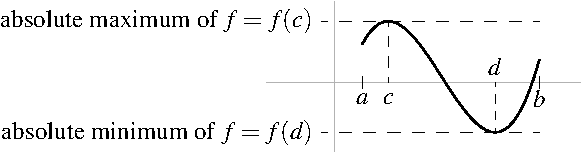
\includegraphics{figures/minmax}
\caption{$f \colon [a,b] \to \R$ achieves an absolute maximum $f(c)$ at
$c$, and an absolute minimum $f(d)$ at $d$.\label{fig:minmax}}
\end{myfigureht}

If $S$ is a closed
and bounded interval, then a continuous $f$
must achieve an absolute minimum and an absolute
maximum on $S$.

\begin{thm}[Minimum-maximum theorem]
\index{Minimum-maximum theorem}
\index{Maximum-minimum theorem}
Let $f \colon [a,b] \to \R$ be a continuous function.  Then $f$
achieves both an absolute minimum and an absolute maximum on $[a,b]$.
\end{thm}

\begin{proof}
The lemma says that $f$ is bounded, and thus
the set $f([a,b]) = \{ f(x) : x \in [a,b] \}$ has a supremum and an infimum.
There exist sequences
in the set $f([a,b])$ that approach its supremum and its infimum.
That is, there are sequences
$\{ f(x_n) \}$ and $\{ f(y_n) \}$, where $x_n, y_n$ are in $[a,b]$,
such that
\begin{equation*}
\lim_{n\to\infty} f(x_n) = \inf f([a,b]) \qquad \text{and} \qquad
\lim_{n\to\infty} f(y_n) = \sup f([a,b]).
\end{equation*}
We are not done yet, we need to find where the minima and the maxima are.
The problem is that the sequences $\{ x_n \}$ and $\{ y_n \}$ need not
converge.
We know $\{ x_n \}$ and $\{ y_n \}$ are bounded (their elements
belong to 
a bounded interval $[a,b]$).
Apply the 
\hyperref[thm:bwseq]{Bolzano--Weierstrass theorem},
to find
convergent subsequences
$\{ x_{n_i} \}$ and 
$\{ y_{m_i} \}$.  Let
\begin{equation*}
x := \lim_{i\to\infty} x_{n_i}
\qquad \text{and} \qquad
y := \lim_{i\to\infty} y_{m_i}.
\end{equation*}
As $a \leq x_{n_i} \leq b$, we have $a \leq x \leq b$,
and similarly $a \leq y \leq b$.  So $x$ and $y$ are in $[a,b]$.
A limit of a subsequence is the same as the limit of the
sequence, and we can take a limit past the continuous function $f$:
\begin{equation*}
\inf f([a,b]) = \lim_{n\to\infty} f(x_n)
= \lim_{i\to\infty} f(x_{n_i}) = 
f \Bigl( \lim_{i\to\infty} x_{n_i} \Bigr) = f(x) .
\end{equation*}
Similarly,
\begin{equation*}
\sup f([a,b]) = \lim_{n\to\infty} f(m_n)
= \lim_{i\to\infty} f(y_{m_i}) = 
f \Bigl( \lim_{i\to\infty} y_{m_i} \Bigr) = f(y) .
\end{equation*}
Therefore, $f$ achieves an absolute minimum at $x$ and
$f$ achieves an absolute maximum at $y$.
\end{proof}

\begin{example}
The function $f(x) := x^2+1$ defined on the interval $[-1,2]$ achieves a minimum
at $x=0$ when $f(0) = 1$.  It achieves a maximum at $x=2$ where $f(2) = 5$.
Do note that the domain of definition matters.  If we instead took the domain
to be $[-10,10]$, then $x=2$ would no longer be a maximum of $f$.  Instead
the maximum would be achieved at either $x=10$ or $x=-10$.
\end{example}

Let us show by examples that the different hypotheses of the theorem are
truly needed.

\begin{example}
The function $f(x) := x$, defined on the whole real line,
achieves neither a minimum, nor a maximum.  So it is important that
we are looking at a bounded interval.
\end{example}

\begin{example}
The function $f(x) := \nicefrac{1}{x}$, defined on $(0,1)$ 
achieves neither a minimum, nor a maximum.  The values of the function are
unbounded as we approach 0.  Also as we approach $x=1$, the values of the
function approach 1, but $f(x) > 1$ for all $x \in (0,1)$.  There is
no $x \in (0,1)$ such that $f(x) = 1$.  So it is important that
we are looking at a closed interval.
\end{example}

\begin{example}
Continuity is important.
Define $f \colon [0,1] \to \R$ by 
$f(x) := \nicefrac{1}{x}$ for $x > 0$ and let $f(0) := 0$.
The function does not achieve a maximum.  The problem is that
the function is not continuous at 0.
\end{example}

\subsection{Bolzano's intermediate value theorem}

Bolzano's intermediate value theorem is one of the cornerstones of analysis.
It is sometimes only called the intermediate value theorem, or just
Bolzano's theorem.  To prove Bolzano's theorem we prove the
following simpler lemma.

\begin{lemma} \label{IVT:lemma}
Let $f \colon [a,b] \to \R$ be a continuous function.
Suppose $f(a) < 0$ and $f(b) > 0$. 
Then there exists a number $c \in (a,b)$
such that $f(c) = 0$.
\end{lemma}

\begin{proof}
We define two sequences $\{ a_n \}$
and $\{ b_n \}$ inductively:
\begin{enumerate}[(i)]
\item Let $a_1 := a$ and $b_1 := b$.
\item If $f\left(\frac{a_n+b_n}{2}\right) \geq 0$, let $a_{n+1} := a_n$ and
$b_{n+1} := \frac{a_n+b_n}{2}$.
\item If $f\left(\frac{a_n+b_n}{2}\right) < 0$, let $a_{n+1} := \frac{a_n+b_n}{2}$ and
$b_{n+1} := b_n$.
\end{enumerate}
\begin{myfigureht}
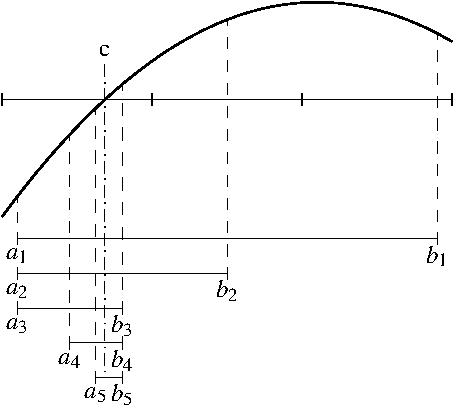
\includegraphics{figures/bisect}
\caption{Finding roots (bisection method).\label{bisectfig}}
\end{myfigureht}
See \figureref{bisectfig} for an example defining the first five steps.
If $a_n < b_n$, then $a_n < \frac{a_n+b_n}{2} < b_n$.  So
$a_{n+1} < b_{n+1}$.
Thus by \hyperref[induction:thm]{induction} $a_n < b_n$ for all $n$.
Furthermore, $a_n \leq a_{n+1}$ and 
$b_n \geq b_{n+1}$ for all $n$, that is the sequences are monotone.
As $a_n < b_n \leq b_1 = b$ and 
$b_n > a_n \geq a_1 = a$ for all $n$,
the sequences are also bounded.  Therefore, the
sequences converge.  Let $c := \lim\, a_n$ and $d := \lim\, b_n$,
where also $a \leq c \leq d \leq b$.  We need
to show that $c=d$.
Notice
\begin{equation*}
b_{n+1} - a_{n+1} = \frac{b_n-a_n}{2}.
\end{equation*}
By \hyperref[induction:thm]{induction},
\begin{equation*}
b_n - a_n = \frac{b_1-a_1}{2^{n-1}} = 2^{1-n} (b-a) .
\end{equation*}
As $2^{1-n}(b-a)$ converges to zero, we take the limit as $n$ goes to
infinity to get
\begin{equation*}
d-c = \lim_{n\to\infty} (b_n - a_n) =
\lim_{n\to\infty} 2^{1-n} (b-a) = 0.
\end{equation*}
In other words $d=c$.

By construction, for all $n$ we have
\begin{equation*}
f(a_n) < 0
\qquad \text{and} \qquad
f(b_n) \geq 0 .
\end{equation*}
Since
$\lim\, a_n = \lim\, b_n = c$
and as $f$ is continuous, we may take 
limits in those inequalities:
\begin{equation*}
f(c) = \lim\, f(a_n) \leq 0
\qquad \text{and} \qquad
f(c) = \lim\, f(b_n) \geq 0 .
\end{equation*}
As $f(c) \geq 0$ and 
$f(c) \leq 0$, we conclude $f(c) = 0$.
Thus also $c \not=a$ and $c \not= b$, so
$a < c < b$.
\end{proof}

\begin{thm}[Bolzano's intermediate value theorem] \label{IVT:thm}
\index{Bolzano's theorem}
\index{Bolzano's intermediate value theorem}
\index{intermediate value theorem}
Let $f \colon [a,b] \to \R$ be a continuous function.
Suppose $y \in \R$ is such that $f(a) < y < f(b)$
or $f(a) > y > f(b)$.  Then there exists a $c \in (a,b)$
such that $f(c) = y$.
\end{thm}

The theorem says that a continuous function on a closed interval
achieves all the values between the values at the endpoints.

\begin{proof}
If $f(a) < y < f(b)$, then define $g(x) := f(x)-y$.  Then we see
that $g(a) < 0$ and $g(b) > 0$ and we apply \lemmaref{IVT:lemma}
to $g$ to find $c$.  If $g(c) = 0$, then $f(c) = y$.

Similarly if $f(a) > y > f(b)$, then define $g(x) := y-f(x)$.  Then
again $g(a) < 0$ and $g(b) > 0$ and we apply \lemmaref{IVT:lemma} to
find $c$.
Again if $g(c) = 0$, then $f(c) = y$.
\end{proof}

If a function is continuous, then the restriction
to a subset is continuous.  So if $f \colon S \to \R$ is continuous and
$[a,b] \subset S$, then $f|_{[a,b]}$ is also continuous.  Hence, we generally
apply the theorem to a function continuous on some large set $S$,
but we restrict attention to an interval.


The proof of the lemma tells us how to find the root $c$.  The
proof is not only useful for us pure mathematicians,
but it is a useful idea in applied mathematics,
where it is called the \emph{\myindex{bisection method}}.


\begin{example}[Bisection method] %\index{bisection method}
The polynomial $f(x) := x^3-2x^2+x-1$ has a real root in $(1,2)$.  We simply
notice that $f(1) = -1$ and $f(2) = 1$.  Hence there must exist a point $c
\in (1,2)$ such that $f(c) = 0$.  To find a better approximation of
the root we follow the proof of \lemmaref{IVT:lemma}.  
We look at 1.5 and find that $f(1.5) = -0.625$.  Therefore,
there is a root of the polynomial in $(1.5,2)$.  Next we look at 1.75
and note that $f(1.75) \approx -0.016$.  Hence there is a root of $f$ in
$(1.75,2)$.  Next we look at 1.875 and find that $f(1.875) \approx 0.44$,
thus there is a root in $(1.75,1.875)$.  We follow this procedure until we gain
sufficient precision.  In fact, the root is at $c \approx 1.7549$.
\end{example}

The technique above is the simplest method of finding roots of polynomials,
which is perhaps the most common problem in applied
mathematics.  In general it is hard to do quickly, precisely,
and automatically.

There are better and faster methods of finding roots of equations, such
as Newton's method.  One advantage of the above method is its
simplicity.  The
moment we find an initial interval where the intermediate value theorem
applies, we are guaranteed to find a root up to a desired
precision in finitely many steps.  Furthermore, the bisection
method finds
roots of any
a continuous function, not just a polynomial.

The theorem guarantees at least one $c$ such that $f(c) = y$, but there
may be many different roots of the equation $f(c) = y$.  If we follow
the procedure of the proof, we are guaranteed to find approximations to
one such root.  We need to work harder to find any other roots.

\medskip

Polynomials of even degree may not have any real roots.  For example,
there is no real number $x$ such that $x^2+1 = 0$.  Odd polynomials, on the
other hand, always have at least one real root.

\begin{prop}
Let $f(x)$ be a polynomial of odd degree.  Then $f$ has a real root.
\end{prop}

\begin{proof}
Suppose $f$ is a polynomial of odd degree $d$.  We write
\begin{equation*}
f(x) = a_d x^d + a_{d-1} x^{d-1} + \cdots + a_1 x + a_0 ,
\end{equation*}
where $a_d \not= 0$.  We divide by $a_d$ to obtain a polynomial
\begin{equation*}
g(x) := x^d + b_{d-1} x^{d-1} + \cdots + b_1 x + b_0 ,
\end{equation*}
where $b_k = \nicefrac{a_k}{a_d}$.
Let us show that $g(n)$ is
positive for some large $n \in \N$.
We first compare the highest order term with the rest:
\begin{equation*}
\begin{split}
\abs{\frac{b_{d-1} n^{d-1} + \cdots + b_1 n + b_0}{n^d}}
& =
\frac{\abs{b_{d-1} n^{d-1} + \cdots + b_1 n + b_0}}{n^d}
\\
& \leq
\frac{\abs{b_{d-1}} n^{d-1} + \cdots + \abs{b_1} n + \abs{b_0}}{n^d}
\\
& \leq
\frac{\abs{b_{d-1}} n^{d-1} + \cdots + \abs{b_1} n^{d-1} + \abs{b_0} n^{d-1}}{n^d}
\\
& =
\frac{n^{d-1}\bigl(\abs{b_{d-1}} + \cdots + \abs{b_1} + \abs{b_0}\bigr)}{n^d}
\\
& =
\frac{1}{n}
\bigl(\abs{b_{d-1}} + \cdots + \abs{b_1} + \abs{b_0}\bigr) .
\end{split}
\end{equation*}
Therefore
\begin{equation*}
\lim_{n\to\infty} \frac{b_{d-1} n^{d-1} + \cdots + b_1 n + b_0}{n^d}
= 0 .
\end{equation*}
Thus there exists an $M \in \N$ such that 
\begin{equation*}
\abs{\frac{b_{d-1} M^{d-1} + \cdots + b_1 M + b_0}{M^d}} < 1 ,
\end{equation*}
which implies
\begin{equation*}
-(b_{d-1} M^{d-1} + \cdots + b_1 M + b_0) < M^d .
\end{equation*}
Therefore $g(M) > 0$.

Next we look at $g(-n)$ for $n \in \N$.  By a similar argument (exercise)
we find that there exists some $K \in \N$ such that
$b_{d-1} {(-K)}^{d-1} + \cdots + b_1 (-K) + b_0 < K^d$
and therefore $g(-K) < 0$ (why?).
In the
proof make sure you use the fact that $d$ is odd.  In particular, 
if $d$ is odd then ${(-n)}^d = -(n^d)$.

We appeal to the intermediate value theorem to find a
$c \in [-K,M]$, such that $g(c) = 0$.  As $g(x) = \frac{f(x)}{a_d}$,
then $f(c) = 0$, and the proof is done.
\end{proof}

\begin{example}
An interesting fact is that there do exist discontinuous functions that have
the intermediate value property.
The function
\begin{equation*}
f(x) :=
\begin{cases}
\sin(\nicefrac{1}{x}) & \text{ if $x \not= 0$,} \\
0 & \text{ if $x=0$,}
\end{cases}
\end{equation*}
is not continuous at 0, however, it has the intermediate value property.
That is, for any $a < b$, and any $y$ such that $f(a) < y < f(b)$
or $f(a) > y > f(b)$,
there exists a $c$ such that $f(y) = c$.
Proof is left as an exercise.
\end{example}

The intermediate value theorem says that if $f \colon [a,b] \to \R$ is
continuous then $f([a,b])$ contains all the values between $f(a)$ and
$f(b)$.  In fact, more is true.  Combining all the results of this section
we can prove the following useful corollary whose proof is left as an exercise.

\begin{cor} \label{cor:imageofinterval}
If $f \colon [a,b] \to \R$ is continuous, then the direct image $f([a,b])$
is a closed and bounded interval or a single number.
\end{cor}

\subsection{Exercises}

\begin{exercise}
Find an example of a discontinuous function $f \colon [0,1] \to \R$
where the intermediate value theorem fails.
\end{exercise}

\begin{exercise}
Find an example of a \emph{bounded} discontinuous function $f \colon [0,1]
\to \R$ that has neither an absolute minimum nor an absolute maximum.
\end{exercise}

\begin{exercise}
Let $f \colon (0,1) \to \R$ be a continuous function such that
$\displaystyle \lim_{x\to 0} f(x) =
\displaystyle \lim_{x\to 1} f(x) = 0$.  Show that
$f$ achieves either an absolute minimum or an absolute maximum on $(0,1)$
(but perhaps not both).
\end{exercise}

\begin{exercise}
Let
\begin{equation*}
f(x) :=
\begin{cases}
\sin(\nicefrac{1}{x}) & \text{ if $x \not= 0$,} \\
0 & \text{ if $x=0$.}
\end{cases}
\end{equation*}
Show that $f$ has the intermediate value property.
That is, for any $a < b$, if there exists a $y$ such that $f(a) < y < f(b)$
or $f(a) > y > f(b)$, then
there exists a $c \in (a,b)$ such that $f(c) = y$.
\end{exercise}

\begin{exercise}
Suppose $g(x)$ is a polynomial of odd degree $d$ such that
\begin{equation*}
g(x) = x^d + b_{d-1} x^{d-1} + \cdots + b_1 x + b_0 ,
\end{equation*}
for some real numbers $b_{0}, b_1, \ldots, b_{d-1}$.  Show that there exists
a $K \in \N$ such that $g(-K) < 0$.  Hint: Make sure to use the fact that
$d$ is odd.  You will have to use that ${(-n)}^d = -(n^d)$.
\end{exercise}

\begin{exercise}
Suppose $g(x)$ is a polynomial of positive even degree $d$ such that
\begin{equation*}
g(x) = x^d + b_{d-1} x^{d-1} + \cdots + b_1 x + b_0 ,
\end{equation*}
for some real numbers $b_{0}, b_1, \ldots, b_{d-1}$.  Suppose 
$g(0) < 0$.  Show that $g$ has at least two distinct real roots.
\end{exercise}

\begin{exercise}
Prove \corref{cor:imageofinterval}:
Suppose $f \colon [a,b] \to \R$ is a continuous function.  Prove
that the direct image $f([a,b])$ is a closed and bounded interval or
a single number.
\end{exercise}

\begin{exercise}
Suppose $f \colon \R \to \R$ is continuous and periodic with period
$P > 0$.  That is, $f(x+P) = f(x)$ for all $x \in \R$.  Show that $f$
achieves an absolute minimum and an absolute maximum.
\end{exercise}

\begin{exercise}[Challenging]
Suppose $f(x)$ is a bounded polynomial,
in other words, there is an $M$ such that $\abs{f(x)} \leq M$
for all $x \in \R$.  Prove that $f$ must be a constant.
\end{exercise}

\begin{exercise}
Suppose $f \colon [0,1] \to [0,1]$ is continuous.  Show that $f$
has a fixed point, in other words, show that there exists an $x \in [0,1]$ such that
$f(x) = x$.
\end{exercise}

\begin{exercise}
Find an example of a continuous bounded function $f \colon \R \to \R$ that does
not achieve an absolute minimum nor an absolute maximum on $\R$.
\end{exercise}

\begin{exercise}
Suppose $f \colon \R \to \R$ is a continuous function such that
$x \leq f(x) \leq x+1$ for all $x \in \R$.  Find $f(\R)$.
\end{exercise}

\begin{exercise}
True/False, prove or find a counterexample.  If $f \colon \R \to
\R$ is a continuous function such that $f|_{\Z}$ is bounded, then $f$
is bounded.
\end{exercise}

\begin{exercise}
Suppose $f \colon [0,1] \to (0,1)$ is a bijection.  Prove that $f$ is not
continuous.
\end{exercise}

\begin{exercise}
Suppose $f \colon \R \to \R$ is continuous.
a)~If there is a $c$ such that $f(c)f(-c) < 0$,
then there is a $d$ such that $f(d) = 0$.
b)~Find a continuous function $f$ such that
$f(\R) = \R$, but $f(x)f(-x) \geq 0$ for all $x \in \R$.
\end{exercise}

\begin{exercise}
Suppose $g(x)$ is a polynomial of even degree $d$ such that
\begin{equation*}
g(x) = x^d + b_{d-1} x^{d-1} + \cdots + b_1 x + b_0 ,
\end{equation*}
Show that $g$ achieves an absolute minimum on $\R$.
\end{exercise}

\begin{exercise}
Suppose $f(x)$ is a polynomial of degree $d$ and 
$f(\R) = \R$.  Show that $d$ is odd.
\end{exercise}

%%%%%%%%%%%%%%%%%%%%%%%%%%%%%%%%%%%%%%%%%%%%%%%%%%%%%%%%%%%%%%%%%%%%%%%%%%%%%%

\sectionnewpage
\section{Uniform continuity}
\label{sec:unifcont}

\sectionnotes{1.5--2 lectures (Continuous extension can be
optional)}

\subsection{Uniform continuity}

We made a fuss of saying that the $\delta$ in the definition of
continuity depended on the point $c$.  There are situations when it is
advantageous to have a $\delta$ independent of any point.  Let
us give a name to this concept.

\begin{defn}
Let $S \subset \R$, and let $f \colon S \to \R$ be a function.
Suppose for any $\epsilon > 0$ there exists a $\delta > 0$
such that whenever $x, c \in S$ and
$\abs{x-c} < \delta$, then $\abs{f(x)-f(c)} < \epsilon$.
Then we say $f$ is \emph{\myindex{uniformly continuous}}.
\end{defn}

It is not hard to see that a uniformly continuous function
must be continuous.
The only difference in the definitions
is that in uniform continuity, for a given $\epsilon > 0$ we pick a $\delta > 0$ that
works for all $c \in S$.  That is, $\delta$ can no longer depend on $c$,
it only depends on $\epsilon$.  The domain of definition
of the function makes a difference now.  A function that is not uniformly
continuous on a larger set, may be uniformly continuous when restricted to a
smaller set.

\begin{example}
$f \colon [0,1] \to \R$, defined by $f(x) := x^2$ is uniformly continuous.

Proof: Note that $0 \leq x,c \leq 1$.  Then
\begin{equation*}
\abs{x^2-c^2} = \abs{x+c}\abs{x-c}
\leq (\abs{x}+\abs{c}) \abs{x-c}
\leq (1+1)\abs{x-c} .
\end{equation*}
Therefore given $\epsilon > 0$, let $\delta := \nicefrac{\epsilon}{2}$.
If $\abs{x-c} < \delta$, then $\abs{x^2-c^2} < \epsilon$.

\medskip

On the other hand, $g \colon \R \to \R$, defined by $g(x) := x^2$ is not uniformly
continuous.

Proof: Suppose it is uniformly continuous, then for all $\epsilon > 0$,
there would exist a $\delta > 0$ such that
if $\abs{x-c} < \delta$, then $\abs{x^2 -c^2} < \epsilon$.
Take $x > 0$ and let
$c := x+\nicefrac{\delta}{2}$.  Write
\begin{equation*}
\epsilon >
\abs{x^2-c^2} = \abs{x+c}\abs{x-c}
=
(2x+\nicefrac{\delta}{2})\nicefrac{\delta}{2} 
\geq 
\delta x .
\end{equation*}
Therefore $x < \nicefrac{\epsilon}{\delta}$ for all $x > 0$, which is a
contradiction.
\end{example}


\begin{example}
The function $f \colon (0,1) \to \R$, defined by $f(x) := \nicefrac{1}{x}$ is not
uniformly continuous.

Proof: Given $\epsilon > 0$, then $\epsilon >
\abs{\nicefrac{1}{x}-\nicefrac{1}{y}}$ holds if and only if
\begin{equation*}
\epsilon >
\abs{\nicefrac{1}{x}-\nicefrac{1}{y}}
=
\frac{\abs{y-x}}{\abs{xy}} 
=
\frac{\abs{y-x}}{xy} ,
\end{equation*}
or
\begin{equation*}
\abs{x-y} < xy \epsilon .
\end{equation*}
Therefore, to satisfy the definition of uniform continuity we would have to
have $\delta \leq xy \epsilon$ for all $x,y$ in $(0,1)$, but that would mean
that $\delta \leq 0$.  Therefore there is no single $\delta > 0$.
\end{example}

We have seen that if $f$ is defined on an interval that is either not closed
or not bounded, then $f$ can be continuous, but not uniformly continuous.
For a closed and bounded interval $[a,b]$, we can, however,
make the following statement.

\begin{thm} \label{unifcont:thm}
Let $f \colon [a,b] \to \R$ be a continuous function.  Then $f$
is uniformly continuous.
\end{thm}

\begin{proof}
We prove the statement by contrapositive.
Suppose $f$ is not uniformly continuous.  We will prove
that there is some
$c \in [a,b]$ where $f$ is not continuous.  Let us negate
the definition of uniformly continuous.
There exists an $\epsilon > 0$
such that for every $\delta > 0$, there exist points $x, y$ in $S$ with
$\abs{x-y} < \delta$ and $\abs{f(x)-f(y)} \geq \epsilon$.

So for the $\epsilon > 0$ above,
we find sequences $\{ x_n \}$ and $\{ y_n \}$ such that
$\abs{x_n-y_n} < \nicefrac{1}{n}$ and such that $\abs{f(x_n)-f(y_n)} \geq
\epsilon$.  By
\hyperref[thm:bwseq]{Bolzano--Weierstrass},
there exists a convergent subsequence
$\{ x_{n_k} \}$.  Let $c := \lim\, x_{n_k}$.
As $a \leq x_{n_k} \leq b$, then $a \leq c \leq b$.  Write
\begin{equation*}
\abs{y_{n_k} - c} =
\abs{y_{n_k} - x_{n_k} + x_{n_k} - c} \leq
\abs{y_{n_k} - x_{n_k}}
+
\abs{x_{n_k}-c}
<
\nicefrac{1}{n_k} 
+
\abs{x_{n_k}-c} .
\end{equation*}
As $\nicefrac{1}{n_k}$ and $\abs{x_{n_k}-c}$ both go to zero when
$k$ goes to infinity, $\{ y_{n_k} \}$ converges and the limit
is $c$.  We now show that $f$ is not continuous at $c$.  We
estimate
\begin{equation*}
\begin{split}
\abs{f(x_{n_k}) - f(c)} & =
\abs{f(x_{n_k}) - f(y_{n_k}) + f(y_{n_k}) - f(c)} \\
& \geq
\abs{f(x_{n_k}) - f(y_{n_k})} - \abs{f(y_{n_k}) - f(c)} \\
& \geq
\epsilon - \abs{f(y_{n_k})-f(c)} .
\end{split}
\end{equation*}
Or in other words
\begin{equation*}
\abs{f(x_{n_k})-f(c)} 
+
\abs{f(y_{n_k})-f(c)}  \geq
\epsilon .
\end{equation*}
At least one of the sequences $\{ f(x_{n_k}) \}$  or
$\{ f(y_{n_k}) \}$ cannot converge to $f(c)$, otherwise the left
hand side of the inequality would go to zero while the right-hand side is positive.
Thus $f$ cannot be continuous at $c$.
\end{proof}

\subsection{Continuous extension}

Before we get to continuous extension, we show the following useful lemma.
It says that uniformly continuous functions behave nicely with respect
to Cauchy sequences.  The new issue here is that for a Cauchy sequence
we no longer know where the limit ends up; it may not end up in the domain
of the function.

\begin{lemma} \label{unifcauchycauchy:lemma}
Let $f \colon S \to \R$ be a uniformly continuous function.  Let
$\{ x_n \}$ be a Cauchy sequence in $S$.  Then $\{ f(x_n) \}$ is Cauchy.
\end{lemma}

\begin{proof}
Let $\epsilon > 0$ be given.  There is a $\delta > 0$ such that
$\abs{f(x)-f(y)} < \epsilon$ whenever $\abs{x-y} < \delta$.  Find an $M
\in \N$ such that for all $n, k \geq M$ we have $\abs{x_n-x_k} < \delta$.
Then for all $n, k \geq M$ we have $\abs{f(x_n)-f(x_k)} < \epsilon$.
\end{proof}

An application of the above lemma is the following result.  It says that
a function on an open interval is uniformly continuous if and only if
it can be extended to a continuous function on the closed interval.

\begin{prop} \label{context:prop}
A function $f \colon (a,b) \to \R$ is uniformly continuous if and only if
the limits 
\begin{equation*}
L_a := \lim_{x \to a} f(x) \qquad \text{and} \qquad
L_b := \lim_{x \to b} f(x)
\end{equation*}
exist and the function $\widetilde{f} \colon [a,b] \to \R$
defined by
\begin{equation*}
\widetilde{f}(x) :=
\begin{cases}
f(x) & \text{ if $x \in (a,b)$,} \\
L_a & \text{ if $x = a$,} \\
L_b & \text{ if $x = b$,}
\end{cases}
\end{equation*}
is continuous.
\end{prop}

\begin{proof}
One direction is not difficult.  If $\widetilde{f}$ is continuous, then
it is uniformly continuous by \thmref{unifcont:thm}.  As $f$ is the
restriction of $\widetilde{f}$ to $(a,b)$, then $f$ is also uniformly continuous
(easy exercise).

Now suppose $f$ is uniformly continuous.  We must first show
that the limits $L_a$ and $L_b$ exist.  Let us concentrate on $L_a$.
Take a sequence $\{ x_n \}$ in $(a,b)$ such that $\lim\, x_n = a$.
The sequence $\{ x_n \}$ is Cauchy, so by
\lemmaref{unifcauchycauchy:lemma}
the sequence $\{ f(x_n) \}$ is Cauchy and thus convergent.
We have some number $L_1 := \lim\, f(x_n)$.  Take another sequence
$\{ y_n \}$ in $(a,b)$ such that $\lim\, y_n = a$.  By the same reasoning
we get $L_2 := \lim\, f(y_n)$.  If we show that $L_1 = L_2$, then
the limit $L_a = \lim_{x\to a} f(x)$ exists.  Let $\epsilon > 0$ be given.
Find $\delta > 0$ such that $\abs{x-y} < \delta$ implies $\abs{f(x)-f(y)} <
\nicefrac{\epsilon}{3}$.  Find $M \in \N$ such that for
$n \geq M$ we have $\abs{a-x_n} < \nicefrac{\delta}{2}$,
$\abs{a-y_n} < \nicefrac{\delta}{2}$,
$\abs{f(x_n)-L_1} < \nicefrac{\epsilon}{3}$, and
$\abs{f(y_n)-L_2} < \nicefrac{\epsilon}{3}$.  Then for $n \geq M$ we have
\begin{equation*}
\abs{x_n-y_n} = 
\abs{x_n-a+a-y_n} \leq
\abs{x_n-a}+\abs{a-y_n} < \nicefrac{\delta}{2} + \nicefrac{\delta}{2} =
\delta.
\end{equation*}
So
\begin{equation*}
\begin{split}
\abs{L_1-L_2} &=
\abs{L_1-f(x_n)+f(x_n)-f(y_n)+f(y_n)-L_2} \\
& \leq 
\abs{L_1-f(x_n)}+\abs{f(x_n)-f(y_n)}+\abs{f(y_n)-L_2} \\
& \leq
\nicefrac{\epsilon}{3} + \nicefrac{\epsilon}{3} + \nicefrac{\epsilon}{3}
=
\epsilon .
\end{split}
\end{equation*}
Therefore $L_1 = L_2$.
Thus $L_a$ exists.  To show that $L_b$ exists is left as an exercise.

Now that we know that the
limits $L_a$ and $L_b$ exist, we are done.  If $\lim_{x\to a} f(x)$
exists, then $\lim_{x\to a} \widetilde{f}(x)$ exists
(See \propref{prop:limrest}).  Similarly with $L_b$.
Hence $\widetilde{f}$ is continuous at $a$ and $b$.  
And since $f$ is continuous at $c \in (a,b)$, then
$\widetilde{f}$ is continuous at $c \in (a,b)$.
\end{proof}

A common application of this proposition (together with
\propref{prop:onesidedlimits})
is the following.
Suppose $f \colon (-1,0) \cup (0,1) \to \R$ is uniformly continuous,
then $\lim_{x\to 0} f(x)$ exists and the function
has what is called an \emph{\myindex{removable singularity}}, that is,
we can extend the function to a continuous function on $(-1,1)$.


\subsection{Lipschitz continuous functions}

\begin{defn}
A function $f \colon S \to \R$
is \emph{\myindex{Lipschitz continuous}}%
\footnote{Named after the German mathematician
\href{http://en.wikipedia.org/wiki/Rudolf_Lipschitz}{Rudolf Otto Sigismund Lipschitz}
(1832--1903).}, if there exists a $K \in \R$, such that
\begin{equation*}
\abs{f(x)-f(y)} \leq K \abs{x-y} 
\qquad \text{for all $x$ and $y$ in $S$.}
\end{equation*}
\end{defn}

A large class of functions is Lipschitz continuous.  Be careful, just as
for uniformly continuous functions, the
domain of definition of the function is important.  See the examples below
and the exercises.  First we justify the use of the word \emph{continuous}.

\begin{prop}
A Lipschitz continuous function is uniformly continuous.
\end{prop}

\begin{proof}
Let $f \colon S \to \R$ be a function and let $K$ be a constant such that
for all $x, y$ in $S$ we have
$\abs{f(x)-f(y)} \leq K \abs{x-y}$.

Let $\epsilon > 0$ be given.  Take $\delta :=
\nicefrac{\epsilon}{K}$.
For any $x$ and $y$ in $S$ such that
$\abs{x-y} < \delta$
we have that
\begin{equation*}
\abs{f(x)-f(y)} \leq K \abs{x-y} < K \delta = K \frac{\epsilon}{K} =
\epsilon .
\end{equation*}
Therefore $f$ is uniformly continuous.
\end{proof}

We interpret Lipschitz continuity geometrically.  If $f$ is a Lipschitz
continuous function with some constant $K$.  We rewrite the inequality 
to say that for $x \not=y$ we have
\begin{equation*}
\abs{\frac{f(x)-f(y)}{x-y}} \leq K .
\end{equation*}
The quantity $\frac{f(x)-f(y)}{x-y}$ is the slope of the line
between the points $\bigl(x,f(x)\bigr)$
and $\bigl(y,f(y)\bigr)$, that is, a \emph{\myindex{secant line}}.  Therefore, $f$ is Lipschitz
continuous if and only if every line that intersects the graph of $f$ in at least two
distinct
points has slope less than or equal to $K$.  See \figureref{fig:lipschitz}.
\begin{myfigureht}
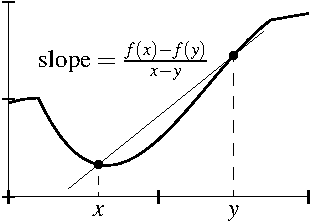
\includegraphics{figures/lipschitzfig}
\caption{The slope of a secant line.
A function is Lipschitz if $\abs{\text{slope}} =
\abs{\frac{f(x)-f(y)}{x-y}} \leq K$ for all $x$ and $y$.\label{fig:lipschitz}}
\end{myfigureht}

\begin{example}
The functions $\sin(x)$ and $\cos(x)$ are Lipschitz continuous.
We have seen (\exampleref{sincos:example}) the following two inequalities.
\begin{equation*}
\abs{\sin(x)-\sin(y)} 
\leq \abs{x-y}
\qquad \text{and} \qquad
\abs{\cos(x)-\cos(y)}
\leq \abs{x-y} .
\end{equation*}

Hence sin and cos are Lipschitz continuous with $K=1$.
\end{example}

\begin{example}
The function $f \colon [1,\infty) \to \R$ defined by $f(x) := \sqrt{x}$
is Lipschitz continuous. Proof:
\begin{equation*}
\abs{\sqrt{x}-\sqrt{y}} = 
\abs{\frac{x-y}{\sqrt{x}+\sqrt{y}}}
=
\frac{\abs{x-y}}{\sqrt{x}+\sqrt{y}} .
\end{equation*}
As $x \geq 1$ and $y \geq 1$, we see that $\frac{1}{\sqrt{x}+\sqrt{y}}
\leq \frac{1}{2}$.  Therefore
\begin{equation*}
\abs{\sqrt{x}-\sqrt{y}} = 
\abs{\frac{x-y}{\sqrt{x}+\sqrt{y}}}
\leq
\frac{1}{2}
\abs{x-y}.
\end{equation*}

On the other hand $f \colon [0,\infty) \to \R$ defined by
$f(x) := \sqrt{x}$ is not Lipschitz continuous.  Let us see why:
Suppose we have
\begin{equation*}
\abs{\sqrt{x}-\sqrt{y}} 
\leq
K \abs{x-y} ,
\end{equation*}
for some $K$.  Let $y=0$ to obtain
$\sqrt{x} \leq K x$.   If $K > 0$, then for $x > 0$ we then get
$\nicefrac{1}{K} \leq \sqrt{x}$.  This cannot possibly be true for all
$x > 0$.  Thus no such $K > 0$ exists and $f$ is not
Lipschitz continuous.

The last example is a function that is uniformly
continuous but not Lipschitz continuous.  To see that $\sqrt{x}$
is
uniformly continuous on $[0,\infty)$ note that it is uniformly continuous on
$[0,1]$ by \thmref{unifcont:thm}.  It is also Lipschitz (and
therefore uniformly continuous) on $[1,\infty)$.  It is not hard (exercise)
to show that this means that $\sqrt{x}$ is uniformly continuous on
$[0,\infty)$.
\end{example}

\subsection{Exercises}

\begin{exercise}
Let $f \colon S \to \R$ be uniformly continuous.  Let $A \subset S$.
Then the restriction $f|_A$ is uniformly continuous.
\end{exercise}

\begin{exercise}
Let $f \colon (a,b) \to \R$ be a uniformly continuous function.
Finish the proof of \propref{context:prop} by showing that
the limit
$\lim\limits_{x \to b} f(x)$
exists.
\end{exercise}

\begin{exercise}
Show that $f \colon (c,\infty) \to \R$ for some $c > 0$
and defined by $f(x) := \nicefrac{1}{x}$ is Lipschitz continuous.
\end{exercise}

\begin{exercise}
Show that $f \colon (0,\infty) \to \R$
defined by $f(x) := \nicefrac{1}{x}$ is not Lipschitz continuous.
\end{exercise}

\begin{exercise}
Let $A, B$ be intervals.
Let $f \colon A \to \R$ and $g \colon B \to \R$ be uniformly continuous
functions such that $f(x) = g(x)$ for $x \in A \cap B$.  Define
the function $h \colon A \cup B \to \R$ by $h(x) := f(x)$ if
$x \in A$ and $h(x) := g(x)$ if $x \in B \setminus A$.
a) Prove that if $A \cap B \not= \emptyset$, then $h$ is uniformly continuous.
b) Find an example where $A \cap B = \emptyset$ and $h$ is not even
continuous.
\end{exercise}

\begin{exercise}[Challenging]
Let $f \colon \R \to \R$ be a polynomial of degree 
$d \geq 2$.  Show that $f$ is not Lipschitz
continuous.
\end{exercise}

\begin{exercise}
Let $f \colon (0,1) \to \R$ be a bounded continuous function.  Show that
the function
$g(x) := x(1-x)f(x)$ is uniformly continuous.
\end{exercise}

\begin{exercise}
Show that $f \colon (0,\infty) \to \R$ defined by $f(x) := \sin
(\nicefrac{1}{x})$ is not uniformly continuous.
\end{exercise}

\begin{exercise}[Challenging]
Let $f \colon \Q \to \R$ be a uniformly continuous function.  Show that
there exists a uniformly continuous function $\widetilde{f} \colon \R \to \R$
such that $f(x) = \widetilde{f}(x)$ for all $x \in \Q$.
\end{exercise}

\begin{exercise}
a) Find a continuous $f \colon (0,1) \to \R$ and a sequence $\{ x_n \}$ in
$(0,1)$ that is Cauchy, but such that $\{ f(x_n) \}$ is not Cauchy.
b) Prove that if $f \colon \R \to \R$ is continuous, and $\{ x_n \}$ is
Cauchy, then $\{ f(x_n) \}$ is Cauchy.
\end{exercise}

\begin{exercise}
a) If $f \colon S \to \R$ and $g \colon S \to \R$ are uniformly continuous,
then show that $h \colon S \to \R$ given by $h(x) := f(x) + g(x)$
is uniformly continuous.\\
b) If $f \colon S \to \R$ is uniformly continuous and $a \in \R$,
then show that $h \colon S \to \R$ given by $h(x) := a f(x)$
is uniformly continuous.
\end{exercise}

\begin{exercise}
a) If $f \colon S \to \R$ and $g \colon S \to \R$ are Lipschitz,
then show that $h \colon S \to \R$ given by $h(x) := f(x) + g(x)$
is Lipschitz.\\
b) If $f \colon S \to \R$ is Lipschitz and $a \in \R$,
then show that $h \colon S \to \R$ given by $h(x) := a f(x)$
is Lipschitz.
\end{exercise}

\begin{exercise}
a) If $f \colon [0,1] \to \R$ is given by $f(x) := x^m$ for an integer
$m \geq 0$,
show $f$ is Lipschitz and find the best (the smallest) Lipschitz constant
$K$ (depending on $m$ of course).
Hint: $(x-y)(x^{m-1} + x^{m-2}y + x^{m-3}y^2 + \cdots + x y^{m-2} + y^{m-1}) = x^m - y^m$.
\\
b) Using the previous exercise, show that if $f \colon [0,1] \to \R$
is a polynomial, that is, $f(x) := a_m x^m + a_{m-1} x^{m-1} + \cdots + a_0$,
then $f$ is Lipschitz.
\end{exercise}

\begin{exercise}
Suppose for $f \colon [0,1] \to \R$ we have $\abs{f(x)-f(y)} \leq K
\abs{x-y}$ for all $x,y$ in $[0,1]$,
and $f(0) = f(1) = 0$.
Prove that $\abs{f(x)} \leq \nicefrac{K}{2}$ for all $x \in [0,1]$.  Further show by example that
$\nicefrac{K}{2}$ is the best possible, that is, there exists such a continuous function
for which $\abs{f(x)} = \nicefrac{K}{2}$ for some $x \in [0,1]$.
\end{exercise}

\begin{exercise}
Suppose $f \colon \R \to \R$ is continuous and periodic with period
$P > 0$.  That is, $f(x+P) = f(x)$ for all $x \in \R$.  Show that $f$
is uniformly continuous.
\end{exercise}

\begin{exercise}
Suppose $f \colon S \to \R$ and $g \colon [0,\infty) \to [0,\infty)$
are functions, $g$ is continuous at $0$, $g(0) = 0$, and
whenever $x$ and $y$ are in $S$ we have $\abs{f(x)-f(y)} \leq g(\abs{x-y})$.
Prove that $f$ is uniformly continuous.
\end{exercise}

\begin{exercise}
Suppose $f \colon [a,b] \to \R$ is a function such that for every $c \in
[a,b]$ there is a $K_c > 0$ and an $\epsilon_c > 0$ for which
$\abs{f(x)-f(y)} \leq K_c \abs{x-y}$ for all $x$ and $y$ in
$(c-\epsilon,c+\epsilon) \cap [a,b]$.  In other words, $f$ is ``locally Lipschitz.''
\\
a)~Prove that there exists a single $K > 0$ such that
$\abs{f(x)-f(y)} \leq K \abs{x-y}$ for all $x,y$ in $[a,b]$.
\\
b)~Find a counterexample to the above if the interval is open, that is,
find an $f \colon (a,b) \to \R$ that is locally Lipschitz, but not
Lipschitz.
\end{exercise}

%%%%%%%%%%%%%%%%%%%%%%%%%%%%%%%%%%%%%%%%%%%%%%%%%%%%%%%%%%%%%%%%%%%%%%%%%%%%%%

\sectionnewpage
\section{Limits at infinity}
\label{sec:limitatinf}

\sectionnotes{less than 1 lecture (optional, can safely be omitted unless
\sectionref{sec:monotonefunc} or
\sectionref{sec:impropriemann} is also covered)}

\subsection{Limits at infinity}

As for sequences, a continuous variable can also approach infinity.  Let
us make this notion precise.

\begin{defn}
We say $\infty$ is a cluster point of $S \subset \R$, if for every
$M \in \R$, there exists an $x \in S$ such that $x \geq M$.  Similarly
$- \infty$ is a cluster point of $S \subset \R$, if for every
$M \in \R$, there exists an $x \in S$ such that $x \leq M$.

\index{limit of a function at infinity}%
Let $f \colon S \to \R$ be a function, where 
$\infty$ is a cluster point of $S$.
If there exists an $L \in \R$
such that for every $\epsilon > 0$, there is an $M \in \R$ such that
\begin{equation*}
\abs{f(x) - L} < \epsilon 
\end{equation*}
whenever $x \geq M$, then we say $f(x)$ \emph{\myindex{converges}} to $L$
as $x$ goes to $\infty$.  We call $L$ the \emph{\myindex{limit}} and write
\begin{equation*}
\lim_{x \to \infty} f(x) := L .
\end{equation*}
Alternatively we write $f(x) \to L$ as $x \to \infty$.

Similarly, if $-\infty$ is a cluster point of $S$
and
there exists an $L \in \R$
such that for every $\epsilon > 0$, there is an $M \in \R$ such that
\begin{equation*}
\abs{f(x) - L} < \epsilon 
\end{equation*}
whenever $x \leq M$, then we say $f(x)$ \emph{converges} to $L$
as $x$ goes to $-\infty$.  We call $L$ the \emph{limit} and write
\begin{equation*}
\lim_{x \to -\infty} f(x) := L .
\end{equation*}
Alternatively we write $f(x) \to L$ as $x \to -\infty$.
\end{defn}

We cheated a little bit again and said \emph{the} limit.
We leave it as an exercise for the reader to prove the following proposition.

\begin{prop} \label{liminfty:unique}
The limit at $\infty$ or $-\infty$ as defined above is unique if it exists.
\end{prop}

\begin{example}
Let $f(x) := \frac{1}{\abs{x}+1}$.  Then
\begin{equation*}
\lim_{x\to \infty} f(x) = 0 \qquad \text{and} \qquad
\lim_{x\to -\infty} f(x) = 0 .
\end{equation*}

Proof:
Let $\epsilon > 0$ be given.  Find $M > 0$ large enough
so that $\frac{1}{M+1} < \epsilon$.  If
$x \geq M$, then $\frac{1}{x+1} \leq \frac{1}{M+1} < \epsilon$.
Since $\frac{1}{\abs{x}+1} > 0$ for all $x$ the first limit is proved.
The proof for $-\infty$ is left to the reader.
\end{example}

\begin{example}
Let $f(x) := \sin(\pi x)$.  Then $\lim_{x\to\infty} f(x)$ does not exist.
To prove this fact note that if $x = 2n+\nicefrac{1}{2}$ for some $n \in \N$ then $f(x)=1$,
while if $x = 2n+\nicefrac{3}{2}$ then $f(x)=-1$, so they cannot both be
within a small $\epsilon$ of a single real number.

We must be careful not to confuse continuous limits with limits of sequences.
We could say
\begin{equation*}
\lim_{n \to \infty} \sin(\pi n) = 0, \qquad \text{but} \qquad
\lim_{x \to \infty} \sin(\pi x) ~ \text{does not exist}.
\end{equation*}
Of course the notation is ambiguous: are we thinking of the
sequence $\{ \sin (\pi n) \}_{n=1}^\infty$ or the function $\sin(\pi x)$
of a real variable.  We are simply using the convention
that $n \in \N$, while $x \in \R$.  When the notation is not clear,
it is good to explicitly mention where the variable lives, or what kind
of limit are you using.  If there is possibility of confusion, one can
write, for example,
\begin{equation*}
\lim_{\substack{n \to \infty\\n \in \N}} \sin(\pi n) .
\end{equation*}
\end{example}

There is a connection of continuous limits to limits of sequences, but we must take all
sequences going to infinity, just as before in \lemmaref{seqflimit:lemma}.

\begin{lemma} \label{seqflimitinf:lemma}
Suppose $f \colon S \to \R$ is a function, $\infty$ is a cluster
point of $S \subset \R$, and $L \in \R$.  Then
\begin{equation*}
\lim_{x\to\infty} f(x) = L
\end{equation*}
if and only if
\begin{equation*}
\lim_{n\to\infty} f(x_n) = L
\end{equation*}
for all sequences $\{ x_n \}$ such that $\lim\limits_{n\to\infty} x_n = \infty$.
\end{lemma}

The lemma holds for the limit as $x \to -\infty$.
Its proof is almost identical and
is left as an exercise.

\begin{proof}
First suppose $f(x) \to L$ as $x \to \infty$.
Given an $\epsilon > 0$, there exists an $M$ such that for all $x \geq M$
we have $\abs{f(x)-L} < \epsilon$.
Let $\{ x_n \}$
be a sequence in $S$ such that $\lim \, x_n = \infty$.  Then there exists an
$N$ such that for all $n \geq N$ we have $x_n \geq M$.  And thus
$\abs{f(x_n)-L} < \epsilon$.

We prove the converse by contrapositive.  Suppose $f(x)$ does
not go to $L$ as $x \to \infty$.
This means that there exists an $\epsilon > 0$,
such that for every $M \in \N$, there exists an $x \in S$, $x \geq M$, let
us call it $x_M$, such that $\abs{f(x_M)-L} \geq \epsilon$.
Consider the sequence $\{ x_n \}$.  Clearly 
$\{ f(x_n) \}$ does not converge to $L$.  It remains to note
that $\lim\, x_n = \infty$, because $x_n \geq n$ for all $n$.
\end{proof}

Using the lemma, we again translate results about sequential
limits into results about continuous limits as $x$ goes to infinity.  That
is, we have almost immediate analogues of the corollaries
in \sectionref{subseq:sequentiallimits}.  We simply allow 
the cluster point $c$ to be either $\infty$ or $-\infty$, in addition
to a real number.  We leave it to
the student to verify these statements.

\subsection{Infinite limit}

Just as for sequences, it is often convenient to distinguish certain
divergent sequences, and talk about limits being infinite
almost as if the limits existed.

\begin{defn}
\index{infinite limit of a function}%
Let $f \colon S \to \R$ be a function and suppose 
$S$ has $\infty$ as a cluster point.
We say $f(x)$
\emph{\myindex{diverges to infinity}} 
as $x$ goes to $\infty$,
if for every $N \in \R$
there exists an $M \in \R$ such that
\begin{equation*}
f(x) > N
\end{equation*}
whenever $x \in S$ and $x \geq M$.
We write
\begin{equation*}
\lim_{x \to \infty} f(x) := \infty ,
\end{equation*}
or we say that $f(x) \to \infty$ as $x \to \infty$.
\end{defn}

A similar definition can be made for limits as $x \to -\infty$
or as $x \to c$ for a finite $c$.  Also similar definitions can be
made for limits being $-\infty$.  Stating these definitions is left
as an exercise.
Note that
sometimes \emph{\myindex{converges to infinity}} is used.
We can again use sequential limits, and an analogue of 
\lemmaref{seqflimit:lemma} is left as an exercise.

\begin{example}
Let us show that $\lim_{x \to \infty} \frac{1+x^2}{1+x} = \infty$.

Proof: For $x \geq 1$ we have
\begin{equation*}
\frac{1+x^2}{1+x} \geq 
\frac{x^2}{x+x}  = 
\frac{x}{2} .
\end{equation*}
Given $N \in \R$, take $M = \max \{ 2N+1 , 1 \}$.
If $x \geq M$, then $x \geq 1$ and $\nicefrac{x}{2} > N$.
So
\begin{equation*}
\frac{1+x^2}{1+x} \geq 
\frac{x}{2} > N .
\end{equation*}
\end{example}

\subsection{Compositions}

Finally, just as for limits at finite numbers we can compose functions
easily.

\begin{prop} \label{prop:inflimcompositions}
Suppose $f \colon A \to B$, $g \colon B \to \R$, $A, B \subset \R$, 
$a \in \R \cup \{ -\infty, \infty\}$ is a cluster point of $A$,
and $b \in \R \cup \{ -\infty, \infty\}$ is a cluster point of $B$.
Suppose 
\begin{equation*}
\lim_{x \to a} f(x) = b\qquad \text{and} \qquad \lim_{y \to b} g(y) = c
\end{equation*}
for some $c \in \R \cup \{ -\infty, \infty \}$.
If $b \in B$, then suppose $g(b) = c$.
Then
\begin{equation*}
\lim_{x \to a} g\bigl(f(x)\bigr) = c .
\end{equation*}
\end{prop}

The proof is straightforward, and left as an exercise.  We already
know the proposition when $a, b, c \in \R$, see Exercises
\ref{exercise:contlimitcomposition} and
\ref{exercise:contlimitbadcomposition}.  Again the requirement that $g$ is
continuous at $b$, if $b \in B$, is necessary.

\begin{example}
Let $h(x) := e^{-x^2+x}$.  Then
\begin{equation*}
\lim_{x\to \infty} h(x) = 0 .
\end{equation*}

Proof:
The claim follows once we know
\begin{equation*}
\lim_{x\to \infty} -x^2+x = -\infty
\end{equation*}
and
\begin{equation*}
\lim_{y\to -\infty} e^y = 0 ,
\end{equation*}
which is usually proved when the exponential function is defined.
\end{example}

\subsection{Exercises}

\begin{exercise}
Prove \propref{liminfty:unique}.
\end{exercise}

\begin{exercise}
Let $f \colon [1,\infty) \to \R$ be a function.  Define
$g \colon (0,1] \to \R$ via $g(x) := f(\nicefrac{1}{x})$.
Using the definitions of limits directly,
show that $\lim_{x\to 0^+} g(x)$
exists if and only if $\lim_{x\to \infty} f(x)$ exists, in which
case they are equal.
\end{exercise}

\begin{exercise}
Prove \propref{prop:inflimcompositions}.
\end{exercise}

\begin{exercise}
Let us justify terminology.
Let $f \colon \R \to \R$ be a function such that
$\lim_{x \to \infty} f(x) = \infty$ (diverges to infinity).
Show that $f(x)$ diverges (i.e.\ does not converge) as $x \to \infty$.
\end{exercise}

\begin{exercise}
Come up with the definitions for limits of $f(x)$ going to $-\infty$ as $x \to
\infty$, $x \to -\infty$, and as $x \to c$ for a finite $c \in \R$.
Then state the definitions for limits of $f(x)$ going to $\infty$ 
as $x \to -\infty$, and as $x \to c$ for a finite $c \in \R$.
\end{exercise}

\begin{exercise}
Suppose $P(x) := x^n + a_{n-1} x^{n-1} + \cdots + a_1 x + a_0$ is a \emph{\myindex{monic polynomial}}
of degree $n \geq 1$ (monic means that the coefficient of $x^n$ is 1). a)
Show that if $n$ is even then $\lim_{x\to\infty} P(x) = 
\lim_{x\to-\infty} P(x) = \infty$.  b)
Show that if $n$ is odd then
$\lim_{x\to\infty} P(x) = \infty$ and
$\lim_{x\to-\infty} P(x) = -\infty$ (see previous exercise).
\end{exercise}

\begin{exercise}
Let $\{ x_n \}$ be a sequence.  Consider $S := \N \subset \R$, and
$f \colon S \to \R$ defined by $f(n) := x_n$.  Show that
the two notions of limit,
\begin{equation*}
\lim_{n\to\infty} x_n \qquad \text{and} \qquad
\lim_{x\to\infty} f(x) 
\end{equation*}
are equivalent.  That is, show that if one exists so does
the other one, and in this case they are equal.
\end{exercise}

\begin{exercise}
Extend \lemmaref{seqflimitinf:lemma} as follows.
Suppose $S \subset \R$ has a cluster point $c \in \R$, $c = \infty$,
or $c = -\infty$.  Let $f \colon S \to \R$ be a function and let
$L = \infty$ or $L = -\infty$.  Show that
\begin{equation*}
\lim_{x\to c} f(x) = L \qquad \text{if and only if} \qquad
\lim_{n\to\infty} f(x_n) = L ~~\text{for all sequences $\{ x_n \}$ such that $\lim\, x_n =
c$} .
\end{equation*}
\end{exercise}

\begin{exercise}
Suppose $f \colon \R \to \R$ is a 2-periodic function, that is $f(x +2) =
f(x)$ for all $x$.  Define $g \colon \R \to \R$ by 
\begin{equation*}
g(x) := f\left(\frac{\sqrt{x^2+1}-1}{x}\right)
\end{equation*}
a)~Find the function $\varphi \colon (-1,1) \to \R$ such that
$g\bigl(\varphi(t)\bigr) = f(t)$, that is $\varphi^{-1}(x) = 
\frac{\sqrt{x^2+1}-1}{x}$.
\\
b)~Show that $f$ is continuous if and only if $g$ is continuous and
\begin{equation*}
\lim_{x \to \infty} g(x) = 
\lim_{x \to -\infty} g(x) = 
f(1) = f(-1) .
\end{equation*}
\end{exercise}

%%%%%%%%%%%%%%%%%%%%%%%%%%%%%%%%%%%%%%%%%%%%%%%%%%%%%%%%%%%%%%%%%%%%%%%%%%%%%%

\sectionnewpage
\section{Monotone functions and continuity}
\label{sec:monotonefunc}

\sectionnotes{1 lecture (optional, can safely be omitted unless
\sectionref{sec:ift} is also covered, requires \sectionref{sec:limitatinf})}

\begin{defn}
Let $S \subset \R$.
We say $f \colon S \to \R$ is \emph{\myindex{increasing}}
(resp.\  \emph{\myindex{strictly increasing}}) if $x,y \in S$ with
$x < y$ implies $f(x) \leq f(y)$ (resp.\ $f(x) < f(y)$).
We define
\emph{\myindex{decreasing}} and
\emph{\myindex{strictly decreasing}} in the same way by switching the
inequalities for $f$.

If a function is either increasing or decreasing we say it is
\emph{monotone}\index{monotone function}.  If it is
strictly increasing or strictly decreasing we say it is
\emph{strictly monotone}\index{strictly monotone function}.
\end{defn}

Sometimes \emph{\myindex{nondecreasing}}
(resp.\ \emph{\myindex{nonincreasing}}) is used
for increasing (resp.\ decreasing) function to emphasize it is not
strictly increasing (resp.\ strictly decreasing).

If $f$ is increasing, then $-f$ is decreasing and vice-versa.  Therefore,
many results about monotone functions can just be proved for say increasing
functions, and the results will follow easily for decreasing functions.

\subsection{Continuity of monotone functions}

It is easy to compute one-sided limits for monotone functions.

\begin{prop} \label{prop:monotlimits}
Let $S \subset \R$, $c \in \R$,
$f \colon S \to \R$ be increasing,
and
$g \colon S \to \R$ be decreasing.
If $c$ is a cluster point of $S \cap (-\infty,c)$, then
\begin{equation*}
\lim_{x \to c^-} f(x) = \sup \{ f(x) : x < c, x \in S \}
\qquad \text{and} \qquad
\lim_{x \to c^-} g(x) = \inf \{ g(x) : x < c, x \in S \} .
\end{equation*}
If $c$ is a cluster point of $S \cap (c,\infty)$, then
\begin{equation*}
\lim_{x \to c^+} f(x) = \inf \{ f(x) : x > c, x \in S \}
\qquad \text{and} \qquad
\lim_{x \to c^+} g(x) = \sup \{ g(x) : x > c, x \in S \} .
\end{equation*}
If $\infty$ is a cluster point of $S$, then
\begin{equation*}
\lim_{x \to \infty} f(x) = \sup \{ f(x) : x \in S \}
\qquad \text{and} \qquad
\lim_{x \to \infty} g(x) = \inf \{ g(x) : x \in S \} .
\end{equation*}
If $-\infty$ is a cluster point of $S$, then
\begin{equation*}
\lim_{x \to -\infty} f(x) = \inf \{ f(x) : x \in S \}
\qquad \text{and} \qquad
\lim_{x \to -\infty} g(x) = \sup \{ g(x) : x \in S \} .
\end{equation*}
\end{prop}

In particular all the one-sided limits exist whenever they make
sense.  For monotone functions therefore, when we say
the left hand limit $x \to c^-$
exists, we mean that $c$ is a cluster point of $S \cap (-\infty,c)$,
and same for the right hand limit.

\begin{proof}
Let us assume $f$ is increasing, and we will show the first
equality.  The rest of the proof is very similar and is left as an
exercise.

Let $a := \sup \{ f(x) : x < c, x \in S \}$.  If $a = \infty$,
then given an $M \in \R$, there exists an $x_M \in S$, $x_M < c$, such that $f(x_M) > M$. 
As $f$ is increasing, $f(x) \geq f(x_M) >  M$ for all $x \in S$ with $x > x_M$.  If
we take $\delta := c-x_M > 0$, then we obtain the definition of the limit going to
infinity.

Next suppose $a < \infty$.
Let $\epsilon > 0$ be given.  Because $a$ is the supremum and
$S \cap (-\infty,c)$ is nonempty, $a \in \R$ and
there exists an
$x_\epsilon \in S$,
$x_\epsilon < c$,
such that $f(x_\epsilon) > a-\epsilon$.  As $f$ is increasing,
if $x \in S$ and $x_\epsilon < x < c$, we have
$a-\epsilon < f(x_\epsilon) \leq f(x) \leq a$.  Let
$\delta := c-x_\epsilon$.  Then for $x \in S \cap (-\infty,c)$
with $\abs{x-c} < \delta$,
we have $\abs{f(x)-a} < \epsilon$.
\end{proof}

Suppose $f \colon S \to \R$, $c \in S$, and
that both one-sided limits exist.
Since $f(x) \leq f(c) \leq f(y)$
whenever $x < c < y$, taking the limits we obtain
\begin{equation*}
\lim_{x \to c^-} f(x) \leq f(c) \leq \lim_{x \to c^+} f(x) .
\end{equation*}
Then $f$ is continuous at $c$ if and only if both limits are equal
to each other (and hence equal to $f(c)$).  See also
\propref{prop:onesidedlimits}.
See \figureref{fig:figinccont} to get an idea of a what a discontinuity
looks like.


\begin{cor} \label{cor:continterval}
If $I \subset \R$ is an interval and $f \colon I \to \R$ is 
monotone and not constant, then $f(I)$ is an interval if and only if $f$
is continuous.
\end{cor}

Assuming $f$ is not constant is to avoid the technicality
that $f(I)$ is a single point in that case; $f(I)$ is a single
point if and only if $f$ is constant.  A constant function is 
continuous.

\begin{proof}
Without loss of generality suppose $f$ is increasing.

First suppose $f$ is continuous.  Take two points
$f(x_1) < f(x_2)$ in $f(I)$.
As $f$ is increasing then $x_1 < x_2$.  By the
\hyperref[IVT:thm]{intermediate value theorem},
given any $y$ with $f(x_1) < y < f(x_2)$, we find
a $c \in (x_1,x_2) \subset I$ such that $f(c) = y$, so $y \in f(I)$. 
Hence, $f(I)$ is an interval.

Let us prove the reverse direction by contrapositive.
Suppose $f$ is not continuous at $c \in I$,
and that $c$ is not an endpoint of $I$.
Let
\begin{equation*}
a := \lim_{x \to c^-} f(x) = \sup \{ f(x) : x \in I, x < c \} ,
\qquad
b := \lim_{x \to c^+} f(x) = \inf \{ f(x) : x \in I, x > c \} .
\end{equation*}
As $c$ is a discontinuity, $a < b$.
If $x < c$, then $f(x) \leq a$, and
if $x > c$, then $f(x) \geq b$.  Therefore
no point
in $(a,b) \setminus \{ f(c) \}$ is in $f(I)$.
However there exists $x_1 \in S$, $x_1 < c$, so
$f(x_1) \leq a$, and there exists $x_2 \in S$, $x_2 > c$,
so $f(x_2) \geq b$.  Both $f(x_1)$ and $f(x_2)$ are in $f(I)$,
but there are points in between them that are not in $f(I)$.
So $f(I)$ is not an interval.  See \figureref{fig:figinccont}.

When $c \in I$ is an endpoint, the proof is similar and is left as an exercise.
\end{proof}

\begin{myfigureht}
\subimport*{figures/}{figinccont.pdf_t}
\caption{Increasing function $f \colon I \to \R$ discontinuity at
$c$.\label{fig:figinccont}}
\end{myfigureht}

A striking property of monotone functions is that they cannot have
too many discontinuities.

\begin{cor} \label{cor:monotcountcont}
Let $I \subset \R$ be an interval and
$f \colon I \to \R$ be monotone.  Then $f$ has at most
countably many discontinuities.
\end{cor}

\begin{proof}
Let $E \subset I$ be the set of all discontinuities
that are not endpoints of $I$.  As there are
only two endpoints, it is enough to show that $E$ is countable.
Without loss of generality, suppose $f$ is increasing.
We will define an injection $h \colon E \to \Q$.
For each $c \in E$
the one-sided limits of $f$ both exist as $c$ is not an endpoint.
Let
\begin{equation*}
a := \lim_{x \to c^-} f(x) = \sup \{ f(x) : x \in I, x < c \} ,
\qquad
b := \lim_{x \to c^+} f(x) = \inf \{ f(x) : x \in I, x > c \} .
\end{equation*}
As $c$ is a discontinuity, we have $a < b$.  
There exists a rational number $q \in (a,b)$, so let $h(c) := q$.
If $d \in E$ is another discontinuity, then if $d > c$, then there
exist an $x \in I$ with $c < x < d$, and so $\lim_{x \to d^-} f(x) \geq b$.
Hence the rational number we choose for $h(d)$ is different from $q$,
since $q=h(c) < b$ and $h(d) > b$.
Similarly if $d < c$.  So after making such a choice for
every $c \in E$, we have a 
one-to-one (injective) function into $\Q$.  Therefore, $E$ is countable.
\end{proof}

\begin{example} \label{example:countdiscont}
By $\lfloor x \rfloor$ denote the largest integer less than or equal to $x$.
Define $f \colon [0,1] \to \R$ by
\begin{equation*}
f(x) :=
x +
\sum_{n=0}^{\lfloor 1/(1-x) \rfloor}
2^{-n} ,
\end{equation*}
for $x < 1$ and $f(1) = 3$.
It is left as an exercise to show that $f$ is strictly increasing, bounded, and
has a discontinuity at all points $1-\nicefrac{1}{k}$ for $k \in \N$.  In particular,
there are countably many discontinuities, but the function is bounded and
defined on a closed bounded interval.  See \figureref{fig:countdiscont}.
\begin{myfigureht}
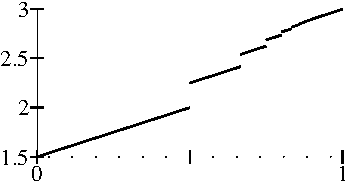
\includegraphics{figures/increasing-discont-fig}
\caption{Increasing function with countably many
discontinuities.\label{fig:countdiscont}}
\end{myfigureht}

Similarly one can find an example of a function discontinuous on a dense set
such as the rational numbers.  See the exercises.
\end{example}


\subsection{Continuity of inverse functions}


A strictly monotone function $f$ is one-to-one (injective).  To see this
notice that if $x \not= y$ then we can assume $x < y$.  Then either $f(x) <
f(y)$ if $f$ is strictly increasing or $f(x) > f(y)$ if $f$ is strictly
decreasing, so $f(x) \not= f(y)$.
Hence, it
must have an inverse $f^{-1}$ defined on its range.

\begin{prop} \label{prop:invcont}
If $I \subset \R$ is an interval and $f \colon I \to \R$ is strictly
monotone.  Then the inverse $f^{-1} \colon f(I) \to I$ is continuous.
\end{prop}

\begin{proof}
Let us suppose $f$ is strictly increasing.  The proof is almost
identical for a strictly decreasing function.
Since $f$ is strictly increasing, so is $f^{-1}$.  That is, if $f(x) <
f(y)$, then we must have $x < y$ and therefore
$f^{-1}\bigl(f(x)\bigr) < f^{-1}\bigl(f(y)\bigr)$.

Take $c \in f(I)$.
If $c$ is not a cluster point of $f(I)$, then $f^{-1}$ is continuous at $c$
automatically.  So let $c$ be a cluster point of $f(I)$.
Suppose both of the following one-sided limits exist:
\begin{align*}
x_0 & := \lim_{y \to c^-} f^{-1}(y) =
\sup \{ f^{-1}(y) : y < c, y \in f(I) \}
=
\sup \{ x \in I : f(x) < c \} , \\
x_1 & := \lim_{y \to c^+} f^{-1}(y) =
\inf \{ f^{-1}(y) : y > c, y \in f(I) \}
=
\inf \{ x \in I : f(x) > c \} .
\end{align*}
We have $x_0 \leq x_1$ as $f^{-1}$ is increasing.
For all $x > x_0$ with $x \in I$, we have $f(x) \geq c$.  As $f$ is strictly increasing,
we must have $f(x) > c$ for all $x > x_0$, $x \in I$.  Therefore,
\begin{equation*}
\{ x \in I : x > x_0 \} \subset \{ x \in I : f(x) > c \}.
\end{equation*}
The infimum of the left hand set is $x_0$, and the infimum of the right hand
set is $x_1$, so we obtain $x_0 \geq x_1$.
So $x_1 = x_0$, and $f^{-1}$ is continuous at $c$.

If one of the one-sided limits does not exist the argument is similar
and is left as an exercise.
\end{proof}

\begin{example}
The proposition does not require $f$ itself to be continuous.  For example, let
$f \colon \R \to \R$
\begin{equation*}
f(x) :=
\begin{cases}
x & \text{if $x < 0$}, \\
x+1 & \text{if $x \geq 0$}. \\
\end{cases}
\end{equation*}
The function $f$ is not continuous at $0$.
The image of $I = \R$ is the set 
$(-\infty,0)\cup [1,\infty)$, not an interval.
Then $f^{-1} \colon (-\infty,0)\cup [1,\infty)
\to \R$ can be written as
\begin{equation*}
f^{-1}(y) =
\begin{cases}
y & \text{if $y < 0$}, \\
y-1 & \text{if $y \geq 1$}. 
\end{cases}
\end{equation*}
It is not difficult to see that $f^{-1}$ is a continuous function.  See
\figureref{invcontfig} for the graphs.
\begin{myfigureht}
\hspace{\fill}
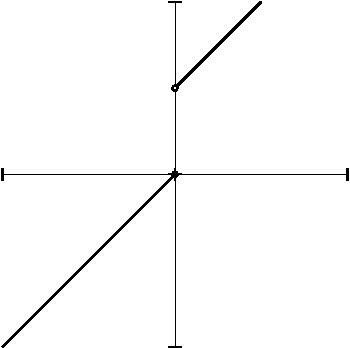
\includegraphics{figures/invcontfigA}
\hspace{\fill}
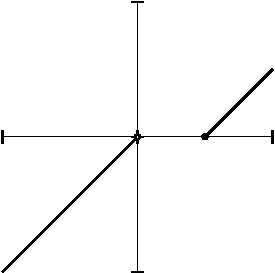
\includegraphics{figures/invcontfigB}
\hspace{\fill}
\caption{Graph of $f$ on the left and $f^{-1}$ on the right.\label{invcontfig}}
\end{myfigureht}
\end{example}

Notice what happens with the proposition if $f(I)$ is an interval.  In that case we could simply
apply \corref{cor:continterval} to both $f$ and $f^{-1}$.  That is, if
$f \colon I \to J$ is an onto strictly monotone function and $I$ and $J$ are intervals,
then both $f$ and $f^{-1}$ are continuous.  Furthermore $f(I)$ is an
interval precisely when $f$ is continuous.

\subsection{Exercises}

\begin{exercise}
Suppose $f \colon [0,1] \to \R$ is monotone.  Prove $f$ is bounded.
\end{exercise}

\begin{exercise}
Finish the proof of \propref{prop:monotlimits}.
Hint: You can halve your work by noticing that if $g$ is decreasing
then $-g$ is increasing.
\end{exercise}

\begin{exercise}
Finish the proof of \corref{cor:continterval}.
\end{exercise}

\begin{exercise}
Prove the claims in \exampleref{example:countdiscont}.
\end{exercise}

\begin{exercise}
Finish the proof of \propref{prop:invcont}.
\end{exercise}

\begin{exercise}
Suppose $S \subset \R$, and $f \colon S \to \R$ is an increasing
function.
a) If $c$ is a cluster point
of $S \cap (c,\infty)$ show that 
$\lim\limits_{x\to c^+} f(x) < \infty$.
b) If $c$ is a cluster point of $S \cap (-\infty,c)$
and $\lim\limits_{x\to c^-} f(x) = \infty$, prove that 
$S \subset (-\infty,c)$.
\end{exercise}

\begin{exercise}
Suppose $I \subset \R$ is an interval and $f \colon I \to \R$ is a function
such that for each $c \in I$, there exist $a, b \in \R$ with
$a > 0$ such that $f(x) \geq a x + b$ for all $x \in I$
and $f(c) = a c + b$.  Show that $f$ is strictly increasing.
\end{exercise}

\begin{exercise}
Suppose $f \colon I \to J$ is a continuous, bijective (one-to-one and onto)
function for two intervals $I$ and $J$.  Show that $f$ is strictly monotone.
\end{exercise}

\begin{exercise}
Consider a monotone function $f \colon I \to \R$ on an interval $I$.  Prove that there exists
a function $g \colon I \to \R$ such that
$\lim\limits_{x \to c^-} g(x) = g(c)$ for all $c \in I$, except the
smaller (left) endpoint of $I$, and such that
$g(x) = f(x)$ for all but countably many $x$.
\end{exercise}

\begin{exercise}
a) Let $S \subset \R$ be any subset.  If $f \colon S \to \R$ is increasing,
then show that there exists an increasing $F \colon \R \to \R$
such that $f(x) = F(x)$ for all $x \in S$.
b) Find an example of a strictly increasing $f \colon S \to \R$ such that
an increasing $F$ as above is never strictly increasing.
\end{exercise}

\begin{exercise}[Challenging] \label{exercise:increasingfuncdiscatQ}
Find an example of an increasing function $f \colon [0,1] \to \R$
that has a discontinuity at each rational number.  Then show that the image
$f([0,1])$ contains no interval.  Hint: Enumerate
the rational numbers and define
the function with a series.
\end{exercise}

\begin{exercise}
Suppose $I$ is an interval and $f \colon I \to \R$ is monotone.
Show that $\R \setminus f(I)$ is a countable union of disjoint intervals.
\end{exercise}

\begin{exercise}
Suppose $f \colon [0,1] \to (0,1)$ is increasing.  Show that for any
$\epsilon > 0$, there exists
a strictly increasing $g \colon [0,1] \to (0,1)$ such that
$g(0) = f(0)$, $f(x) \leq g(x)$ for all $x$, and $g(1)-f(1) < \epsilon$.
\end{exercise}

\begin{exercise}
Prove that the Dirichlet function $f \colon [0,1] \to\R$ defined by $f(x) :=
1$ if $x$ is rational and $f(x) := 0$ otherwise cannot be written as a
difference of two increasing functions.  That is, there do not exist
increasing $g$ and $h$ such that, $f(x) = g(x) - h(x)$.
\end{exercise}

\begin{exercise}
Suppose $f \colon (a,b) \to (c,d)$ is a strictly increasing
onto function.  Prove that there exists a $g \colon (a,b) \to (c,d)$,
which is also strictly increasing and onto, and $g(x) < f(x)$ for all $x \in
(a,b)$.
\end{exercise}


